\section{Campaign details}
\label{app:campaign}

This appendix lists the checkpoints and their consumed loci, the acceptance decisions, the coverage of the campaign, and the per-concept results of every completed block.

\subsection{Labels, registration, and artifact}
\label{app:cf-labels}

\paragraph{Labels.} We use each dataset's supplied report-derived labels: NIH ChestX-ray14 finding labels \citep{wang2017chestxray}, the CheXpert labeler output \citep{irvin2019chexpert} distributed with CheXpert Plus \citep{chambon2024chexpertplus}, and COCO instance annotations \citep{lin2014coco}. Rows are positive for label 1, negative for label 0, and \emph{unknown} when the labeler output is uncertain or blank, which is the uncertainty convention of the CheXpert labeler \citep{irvin2019chexpert}. We exclude unknown rows from probe fitting, selectivity, and answer AUROC. We write and score them like all other rows. Fixed manifests drawn with recorded seeds define the cohorts, one manifest per dataset for every block. No patient and no image appears in two roles of a dataset. Every cohort is disjoint from every pilot-study cohort. Three cohorts are scored: the training cohort for fitting the scaler, probes, and answer direction; the 400-row calibration cohort for the readable and answerable grades; and the 600-row test cohort for every write. A second CheXpert cohort contains \cfValidRows{} frontal films from the CheXpert validation set, one per patient, with the radiologists' consensus labels \citep{irvin2019chexpert}. This cohort has zero patient overlap with any campaign cohort.

\paragraph{Registration.} We froze the protocol before scoring any grid block. The loci, projection and probe settings, dose, reference family, six templates, module set, seven gates, and three decision rules match the registered protocol file. We registered the pilot study's crossover and confirmation analyses before running them (Appendix~\ref{app:seed}). After completing the grid, we added the leaderboard, write-flow share, and per-image examples as descriptive summaries of these outputs.

\paragraph{Artifact.} The release includes evaluation code, adapters, the registered protocol file, cohort manifests with their seeds, and fitted directions. It provides per-image outcomes for every module (write, dose, refit, locus, and template rows), scorecards and coverage files for every block, and rendered prompts. Each new checkpoint requires one adapter that identifies its input block and passes the gates.

\subsection{Grid and consumed loci}
\label{app:cf-grid}

\begin{table}[h]
\centering
\setlength{\tabcolsep}{3pt}
% terracotta = positive / high, blue = negative / low, sage = magnitude of Read and Ans; darker = larger magnitude
\definecolor{cfSage1}{HTML}{ECF3EF}
\definecolor{cfSage2}{HTML}{D5E5DB}
\definecolor{cfSage3}{HTML}{B9D4C3}
\definecolor{cfSage4}{HTML}{9EC3AC}
\definecolor{cfSlate1}{HTML}{EAF0F6}
\definecolor{cfSlate2}{HTML}{D0DDEA}
\definecolor{cfSlate3}{HTML}{B1C7DD}
\definecolor{cfSlate4}{HTML}{94B2D0}
\definecolor{cfTerra1}{HTML}{F7ECEA}
\definecolor{cfTerra2}{HTML}{EED5D1}
\definecolor{cfTerra3}{HTML}{E2B8B2}
\definecolor{cfTerra4}{HTML}{D79E95}
\definecolor{cfOat1}{HTML}{F4EFE6}
\definecolor{cfOat2}{HTML}{E8DDC8}
\definecolor{cfGrey}{HTML}{E4E1DC}

\caption{\textbf{Checkpoints and families.} Per checkpoint: vision tower, consumed tokens per image, input size, and eligible templates. Bold family rows give mean selectivity and clean-answer AUROC over clinical cells and the owned clinical and COCO cells, shaded by owned share.}
\label{tab:cf-models}
\resizebox{\linewidth}{!}{%
\begin{tabular}{lllll@{\hspace{8pt}}rrrr}
\toprule
\multirow{2}{*}{Checkpoint} & \multirow{2}{*}{Vision tower} & \multirow{2}{*}{Tokens} & \multirow{2}{*}{Image} & \multirow{2}{*}{Templates} & \multirow{2}{*}{$\bar S$} & \multirow{2}{*}{$\overline{\mathrm{AUROC}}$} & \multicolumn{2}{c}{owned cells}\\
\cmidrule(lr){8-9}
&  &  &  &  &  &  & \multicolumn{1}{c}{clinical} & \multicolumn{1}{c}{COCO}\\
\midrule
\multicolumn{5}{l}{\textbf{Qwen2.5-VL}~\citep{bai2025qwen25vl}} & 0.132 & 0.635 & \cellcolor{cfTerra2}5/48 & \cellcolor{cfTerra4}24/24 \\
\quad Qwen2.5-VL-3B & native ViT 675M & 576$\to$144 & $336^2$ & IYWYIAWA & & & & \\
\quad Qwen2.5-VL-7B & native ViT 675M & 576$\to$144 & $336^2$ & all & & & & \\
\quad Qwen2.5-VL-32B & native ViT 675M & 576$\to$144 & $336^2$ & all & & & & \\
\quad Qwen2.5-VL-72B & native ViT 675M & 576$\to$144 & $336^2$ & all & & & & \\
\midrule
\multicolumn{5}{l}{\textbf{Qwen3-VL}~\citep{qwen2025qwen3vl}} & 0.137 & 0.735 & \cellcolor{cfTerra2}4/36 & \cellcolor{cfTerra4}18/18 \\
\quad Qwen3-VL-4B & SigLIP2-based & $\leq$1024 & $\leq 512^2$ & all & & & & \\
\quad Qwen3-VL-8B & SigLIP2-based & $\leq$1024 & $\leq 512^2$ & all & & & & \\
\quad Qwen3-VL-32B & SigLIP2-based & $\leq$1024 & $\leq 512^2$ & all & & & & \\
\midrule
\multicolumn{5}{l}{\textbf{InternVL3.5}~\citep{wang2025internvl35}} & 0.125 & 0.807 & \cellcolor{cfTerra2}5/36 & \cellcolor{cfTerra4}17/18 \\
\quad InternVL3.5-8B & InternViT-300M & 1024 & $448^2$ & all & & & & \\
\quad InternVL3.5-14B & InternViT-300M & 1024 & $448^2$ & all & & & & \\
\quad InternVL3.5-38B & InternViT-6B & 1024 & $448^2$ & all & & & & \\
\midrule
\multicolumn{5}{l}{\textbf{Gemma 3}~\citep{gemma2025gemma3}} & 0.124 & 0.564 & \cellcolor{cfTerra2}2/36 & \cellcolor{cfTerra4}17/18 \\
\quad Gemma 3 4B & SigLIP-So400m & 4096 & $896^2$ & all & & & & \\
\quad Gemma 3 12B & SigLIP-So400m & 4096 & $896^2$ & all & & & & \\
\quad Gemma 3 27B & SigLIP-So400m & 4096 & $896^2$ & all & & & & \\
\midrule
\multicolumn{5}{l}{\textbf{MedGemma} (medical)~\citep{sellergren2025medgemma}} & 0.164 & 0.835 & \cellcolor{cfTerra2}2/24 & \cellcolor{cfTerra3}10/12 \\
\quad MedGemma 4B & MedSigLIP & 4096 & $896^2$ & all & & & & \\
\quad MedGemma 27B & MedSigLIP & 4096 & $896^2$ & all & & & & \\
\midrule
\multicolumn{5}{l}{\textbf{Lingshu} (medical)~\citep{lasa2025lingshu}} & 0.142 & 0.820 & \cellcolor{cfTerra4}11/24 & \cellcolor{cfTerra4}12/12 \\
\quad Lingshu 7B & Qwen2.5-VL ViT & 576$\to$144 & $336^2$ & all & & & & \\
\quad Lingshu 32B & Qwen2.5-VL ViT & 576$\to$144 & $336^2$ & all & & & & \\
\midrule
\multicolumn{5}{l}{\textbf{LLaVA-1.5}~\citep{liu2024improved}} & 0.124 & 0.516 & \cellcolor{cfTerra1}0/24 & \cellcolor{cfTerra3}7/12 \\
\quad LLaVA-1.5-7B & CLIP ViT-L/14-336 & 576 & $336^2$ & IYWY & & & & \\
\quad LLaVA-1.5-13B & CLIP ViT-L/14-336 & 576 & $336^2$ & IYWYIAWA & & & & \\
\midrule
\multicolumn{5}{l}{\textbf{LLaVA-Med} (medical)~\citep{li2023llavamed}} & 0.136 & 0.560 & \cellcolor{cfTerra2}1/12 & \cellcolor{cfTerra2}1/6 \\
\quad LLaVA-Med 1.5 7B & CLIP ViT-L/14-336 & 576 & $336^2$ & IYWY & & & & \\
\midrule
\multicolumn{5}{l}{\textbf{Llama 3.2 Vision}~\citep{meta2024llama32vision}} & 0.119 & 0.688 & \cellcolor{cfTerra1}0/12 & \cellcolor{cfTerra2}1/6 \\
\quad Llama 3.2 Vision 11B & ViT-H/14 & 1601 & $560^2$ & IBWB & & & & \\
\midrule
\multicolumn{5}{l}{\textbf{CheXagent} (medical)~\citep{chen2024chexagent}} & 0.180 & 0.857 & \cellcolor{cfTerra3}7/24 & \cellcolor{cfTerra2}2/12 \\
\quad CheXagent-2-3B & XraySigLIP ViT-L/16 & 1024 & $512^2$ & IYWYIAWA & & & & \\
\quad CheXagent-8B & EVA-CLIP ViT 1.4B & 1025$\to$128 & $448^2$ & IYWYIAWA & & & & \\
\midrule
\multicolumn{5}{l}{\textbf{LLaVA-Rad} (medical)~\citep{zambranochaves2025llavarad}} & 0.209 & 0.793 & \cellcolor{cfTerra1}0/12 & \cellcolor{cfTerra1}0/6 \\
\quad LLaVA-Rad-7B & BiomedCLIP-CXR-518 & 1369 & $518^2$ & IYWY & & & & \\
\midrule
\multicolumn{5}{l}{\textbf{HuatuoGPT-Vision} (medical)~\citep{chen2024huatuogptvision}} & 0.136 & 0.746 & \cellcolor{cfTerra2}1/12 & \cellcolor{cfTerra3}4/6 \\
\quad HuatuoGPT-Vision-7B & CLIP ViT-L/14-336 & 576 & $336^2$ & all & & & & \\
\bottomrule
\end{tabular}}
\end{table}

\begin{figure}[h]
    \centering
    \resizebox{\textwidth}{!}{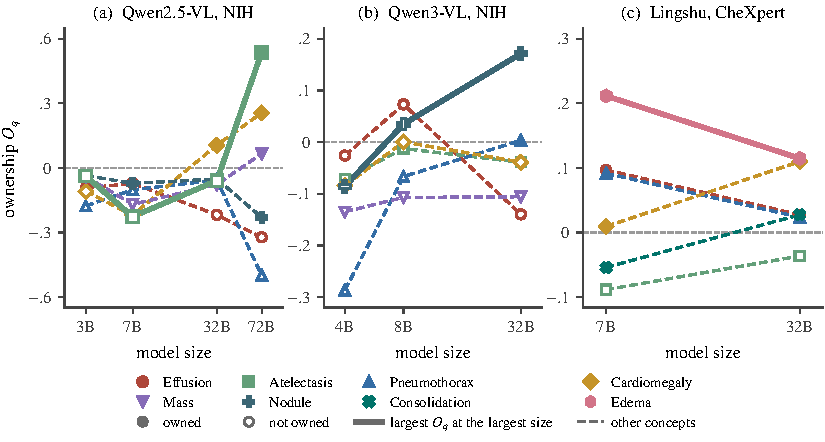
\includegraphics{figures/fig6_ladders.pdf}}
    \caption{\textbf{Size ladders.} Ownership $O_q$ per concept across sizes for Qwen2.5-VL and Qwen3-VL on NIH and Lingshu on CheXpert. Solid lines mark the concept with the largest ownership at the largest size (Atelectasis, Nodule, Edema), filled markers owned cells; vertical scales differ by panel.}
    \label{fig:ladders}
\end{figure}


The towers include CLIP \citep{radford2021clip} in the LLaVA families, SigLIP \citep{zhai2023siglip} in Gemma~3, and a SigLIP~2 design \citep{tschannen2025siglip2} in Qwen3-VL; MedGemma's MedSigLIP tower is a medically tuned SigLIP released with that model \citep{sellergren2025medgemma}. The three towers trained on chest radiographs are the XraySigLIP tower of CheXagent-2-3B \citep{chen2024chexagent}, the EVA-CLIP tower \citep{sun2023evaclip} of CheXagent-8B, and the BiomedCLIP-CXR tower of LLaVA-Rad-7B \citep{zhang2025biomedclip,zambranochaves2025llavarad}; HuatuoGPT-Vision-7B tunes on medical data over the same stock CLIP tower as LLaVA-1.5. Consumed-token counts range from \cfTokensMin{} to \cfTokensMax{} per image, and each family uses a fixed image resolution. The Llama~3.2 Vision projector also reads five intermediate local-layer outputs that bypass the final global block. LLaVA computes the final CLIP block but consumes the penultimate block. At every checkpoint, Gate (C) verifies that the write reaches the consumer and the answer logits and changes nothing outside the consumed tokens.

\subsection{Acceptance decisions}
\label{app:cf-gates}

Seven checks run on the 16 preflight rows at both loci before a block is scored: (A) bitwise determinism; (B) identity at $\alpha=0$; (C) reach, under which the write must change the consumer's input and answer logits without changing anything outside the consumed tokens; (D) batched-versus-single agreement of the answer logits within $0.25$; (E) image-free semantic mapping of every template; (F) throughput; and (G) fp32 recomputation of the answer logits. Deviations in (D) are declared and neutralised by scoring every condition of a question in one fixed batch composition. Templates that fail (E) are ineligible; a checkpoint whose yes/no template fails is graded on its eligible B-positive template (IB for Llama~3.2 Vision), and its scorecards record the template used and every declared deviation.

All \cfWriteBlocks{} completed blocks pass checks (A), (B), (C), and (G): determinism error is zero, change at $\alpha=0$ is zero, and fp32-versus-model logit differences are below \cfGateFpMax{}. In check (D), the Qwen3-VL, Gemma~3, MedGemma, InternVL, and Llama families exceed the 0.25-logit tolerance (up to \cfGateBatchMax{} logits for Gemma~3 12B). We record these as declared deviations. Fixed batch composition neutralises them. Check (E) fails across all datasets for the A/B templates for LLaVA-1.5-7B and LLaVA-Med, the B-mapped templates for Qwen2.5-VL-3B and LLaVA-1.5-13B, and the yes/no and A-mapped templates for Llama~3.2 Vision 11B. We record affected cells as ineligible. Check (E) fails for every template of MAIRA-2 \citep{bannur2024maira} on NIH: the model answers ``No'' to every finding on all \cfSpecUngradedRows{} preflight images and ``A'' to every forced choice under both letter mappings, so no template carries a graded answer and the block produces no outcomes. Two Gemma~3 checkpoints answer ``yes'' to most chest questions; Gemma~3 4B does so on \cfGemmaFourYesMin--\cfGemmaFourYesMax\% of rows (clean $P(\mathrm{yes})>0.99$). The answerability grade records this behaviour. Three checkpoints (LLaVA-1.5 7B/13B, LLaVA-Med) answer at chance.

\subsection{Coverage and cost}
\label{app:cf-coverage}

Every checkpoint has a completed core write matrix and calibration pass on NIH ChestX-ray14, CheXpert Plus, and COCO. The campaign targets \cfCoveragePlannedWord{} modules per block: the write matrix, the calibration pass, the five additional templates, the dose sweep, the two probe refits, the connector locus, and the connector-locus calibration. \cfCoverageBlocksAllSeven{} of \cfBlocks{} blocks carry all seven modules. A probe-graded block whose write matrix is ineligible or incomplete contributes readability alone. Each block's scorecard also reports the dose range of $O_q$ over $\alpha\in[-0.5,0.5]$, its standard deviation over the three fit seeds, ownership at the connector locus, and the wording and mapping contrasts of $O_q$ across the six templates. The partial block is Qwen2.5-VL-72B on CheXpert Plus, which lacks the additional templates and the connector locus. The campaign used about 3,000 A100-hours; a chest block of a 7B checkpoint takes about ten.


\subsection{Ownership of every concept}
\label{app:cf-tables}

Tables~\ref{tab:cf-own-nih}--\ref{tab:cf-own-coco} report the ownership contrast $O_q$ of every concept cell, one table per dataset, with the checkpoints in the order of Table~\ref{tab:cf-main}. Their cells are shaded by magnitude at $0.02$, $0.10$, and $0.25$, terracotta for positive and blue for negative ownership.

\paragraph{NIH ChestX-ray14.} \cfNihOwned{} of the \cfNihCells{} cells are owned, a stronger competitor is identified in \cfNihCompetitor{}, and the contrast is positive in \cfGeoOwnWinsNihPct\% of cells. The owned cells concentrate in a few rows: Qwen2.5-VL-72B owns Atelectasis ($O_q=\cfOQwenSeventyTwoAtel$), Cardiomegaly, and Mass, while in Gemma~3 12B the competing directions win most answers, down to $O_{\mathrm{Effusion}}=\cfOGemmaTwelveEff$.

\begin{table}[htbp]
\centering
\setlength{\tabcolsep}{4pt}
\caption{\textbf{Ownership of every concept, NIH ChestX-ray14.} $O_q$ at $\alpha=+0.25$: bold is owned and $\dagger$ marks a stronger competitor among the cells that clear the reference; the last row counts owned cells. Shading darkens with $|O_q|$ (terracotta positive, blue negative).}
\label{tab:cf-own-nih}
\fitwidth{%
\begin{tabular}{lrrrrrr}
\toprule
Checkpoint & \multicolumn{1}{c}{Effusion} & \multicolumn{1}{c}{Atelectasis} & \multicolumn{1}{c}{Pneumothorax} & \multicolumn{1}{c}{Cardiomegaly} & \multicolumn{1}{c}{Mass} & \multicolumn{1}{c}{Nodule}\\
\midrule
Lingshu 32B & \cellcolor{cfSlate1}-0.01 & \cellcolor{cfSlate2}-0.08 & \cellcolor{cfTerra3}\textbf{+0.14} & \cellcolor{cfTerra2}\textbf{+0.05} & \cellcolor{cfSlate2}-0.08 & \cellcolor{cfSlate3}-0.18 \\
CheXagent-2-3B & \cellcolor{cfSlate1}-0.00$^{\dagger}$ & \cellcolor{cfTerra2}\textbf{+0.04} & \cellcolor{cfSlate1}-0.00$^{\dagger}$ & \cellcolor{cfSlate1}-0.01 & \cellcolor{cfTerra1}\textbf{+0.01} & \cellcolor{cfSlate1}-0.01 \\
Lingshu 7B & \cellcolor{cfTerra1}+0.02 & \cellcolor{cfTerra1}+0.01 & \cellcolor{cfTerra1}+0.01 & \cellcolor{cfTerra3}\textbf{+0.17} & \cellcolor{cfSlate2}-0.09 & \cellcolor{cfTerra1}+0.02 \\
Qwen2.5-VL-72B & \cellcolor{cfSlate4}-0.32 & \cellcolor{cfTerra4}\textbf{+0.54} & \cellcolor{cfSlate4}-0.50 & \cellcolor{cfTerra4}\textbf{+0.26} & \cellcolor{cfTerra2}\textbf{+0.07} & \cellcolor{cfSlate3}-0.23 \\
Qwen3-VL-32B & \cellcolor{cfSlate3}-0.14 & \cellcolor{cfSlate2}-0.04 & \cellcolor{cfTerra1}\textbf{+0.00} & \cellcolor{cfSlate2}-0.04 & \cellcolor{cfSlate3}-0.11 & \cellcolor{cfTerra3}\textbf{+0.17} \\
InternVL3.5-38B & \cellcolor{cfTerra1}\textbf{+0.00} & \cellcolor{cfSlate1}-0.02 & \cellcolor{cfSlate1}-0.00 & \cellcolor{cfSlate2}-0.03 & \cellcolor{cfTerra1}+0.02 & \cellcolor{cfTerra1}+0.00 \\
Qwen3-VL-4B & \cellcolor{cfSlate2}-0.03$^{\dagger}$ & \cellcolor{cfSlate2}-0.07 & \cellcolor{cfSlate4}-0.29 & \cellcolor{cfSlate2}-0.08 & \cellcolor{cfSlate3}-0.13 & \cellcolor{cfSlate2}-0.09 \\
InternVL3.5-14B & \cellcolor{cfTerra1}\textbf{+0.01} & \cellcolor{cfSlate1}-0.01 & \cellcolor{cfSlate1}-0.00 & \cellcolor{cfSlate1}-0.00 & \cellcolor{cfTerra1}+0.00 & \cellcolor{cfSlate1}-0.01 \\
Gemma 3 12B & \cellcolor{cfSlate4}-0.83 & \cellcolor{cfSlate4}-0.57 & \cellcolor{cfSlate3}-0.17 & \cellcolor{cfSlate3}-0.19 & \cellcolor{cfSlate4}-0.65 & \cellcolor{cfTerra3}\textbf{+0.17} \\
Gemma 3 27B & \cellcolor{cfSlate2}-0.04 & \cellcolor{cfSlate2}-0.03 & \cellcolor{cfSlate1}-0.01 & \cellcolor{cfTerra1}\textbf{+0.00} & \cellcolor{cfSlate2}-0.08 & \cellcolor{cfSlate1}-0.02 \\
MedGemma 4B & \cellcolor{cfTerra1}+0.01 & \cellcolor{cfSlate4}-0.56 & \cellcolor{cfTerra1}+0.01 & \cellcolor{cfSlate2}-0.07 & \cellcolor{cfSlate4}-0.27 & \cellcolor{cfTerra2}+0.09 \\
Qwen2.5-VL-32B & \cellcolor{cfSlate3}-0.22 & \cellcolor{cfSlate2}-0.06 & \cellcolor{cfSlate2}-0.06 & \cellcolor{cfTerra3}\textbf{+0.11} & \cellcolor{cfSlate2}-0.08 & \cellcolor{cfSlate2}-0.05 \\
InternVL3.5-8B & \cellcolor{cfTerra1}+0.00 & \cellcolor{cfSlate1}-0.02 & \cellcolor{cfSlate1}-0.00 & \cellcolor{cfTerra1}+0.00 & \cellcolor{cfSlate1}-0.01 & \cellcolor{cfSlate1}-0.01 \\
HuatuoGPT-Vision-7B & \cellcolor{cfSlate2}-0.04 & \cellcolor{cfSlate2}-0.03 & \cellcolor{cfSlate2}-0.03 & \cellcolor{cfSlate2}-0.08 & \cellcolor{cfSlate2}-0.04 & \cellcolor{cfTerra1}\textbf{+0.01} \\
LLaVA-Med 1.5 7B & \cellcolor{cfSlate1}-0.00 & \cellcolor{cfSlate1}-0.00 & \cellcolor{cfSlate2}-0.04 & \cellcolor{cfSlate1}-0.01 & \cellcolor{cfSlate1}-0.01 & \cellcolor{cfSlate2}-0.02 \\
CheXagent-8B & \cellcolor{cfTerra1}+0.01 & \cellcolor{cfSlate1}-0.01 & \cellcolor{cfSlate1}-0.00 & \cellcolor{cfSlate1}-0.00 & \cellcolor{cfTerra1}+0.00 & \cellcolor{cfSlate1}-0.01 \\
Qwen2.5-VL-3B & \cellcolor{cfSlate2}-0.09 & \cellcolor{cfSlate2}-0.04 & \cellcolor{cfSlate3}-0.18 & \cellcolor{cfSlate3}-0.11 & \cellcolor{cfSlate2}-0.04 & \cellcolor{cfSlate2}-0.04 \\
Qwen2.5-VL-7B & \cellcolor{cfSlate2}-0.07$^{\dagger}$ & \cellcolor{cfSlate3}-0.23 & \cellcolor{cfSlate3}-0.10 & \cellcolor{cfSlate3}-0.22 & \cellcolor{cfSlate3}-0.17 & \cellcolor{cfSlate2}-0.07 \\
Qwen3-VL-8B & \cellcolor{cfTerra2}+0.07 & \cellcolor{cfSlate1}-0.01 & \cellcolor{cfSlate2}-0.07 & \cellcolor{cfTerra1}+0.00 & \cellcolor{cfSlate3}-0.11 & \cellcolor{cfTerra2}+0.03 \\
Gemma 3 4B & \cellcolor{cfSlate1}-0.00 & \cellcolor{cfSlate1}-0.00 & \cellcolor{cfSlate1}-0.01 & \cellcolor{cfSlate3}-0.24 & \cellcolor{cfSlate4}-0.28 & \cellcolor{cfSlate3}-0.12 \\
LLaVA-1.5-7B & \cellcolor{cfSlate2}-0.03 & \cellcolor{cfSlate1}-0.01 & \cellcolor{cfSlate2}-0.08 & \cellcolor{cfSlate3}-0.13 & \cellcolor{cfTerra2}+0.02 & \cellcolor{cfSlate1}-0.02 \\
MedGemma 27B & \cellcolor{cfSlate2}-0.06 & \cellcolor{cfSlate4}-0.45 & \cellcolor{cfSlate1}-0.01 & \cellcolor{cfTerra1}+0.00 & \cellcolor{cfSlate3}-0.13 & \cellcolor{cfSlate3}-0.20 \\
LLaVA-1.5-13B & \cellcolor{cfSlate1}-0.01 & \cellcolor{cfSlate2}-0.05 & \cellcolor{cfSlate2}-0.04 & \cellcolor{cfSlate2}-0.03 & \cellcolor{cfTerra1}+0.01 & \cellcolor{cfSlate1}-0.02 \\
Llama 3.2 Vision 11B & \cellcolor{cfSlate2}-0.04 & \cellcolor{cfSlate2}-0.07 & \cellcolor{cfSlate2}-0.05 & \cellcolor{cfTerra2}+0.02 & \cellcolor{cfSlate2}-0.06 & \cellcolor{cfSlate1}-0.01 \\
LLaVA-Rad-7B & \cellcolor{cfSlate1}-0.02 & \cellcolor{cfSlate1}-0.01 & \cellcolor{cfSlate1}-0.00 & \cellcolor{cfTerra1}+0.00 & \cellcolor{cfSlate1}-0.01 & \cellcolor{cfSlate2}-0.03 \\
\midrule
\textbf{Owned} & 2 & 2 & 2 & 5 & 2 & 3 \\
\bottomrule
\end{tabular}}
\end{table}

\begin{table}[htbp]
\centering
\setlength{\tabcolsep}{4pt}
\caption{\textbf{Ownership of every concept, CheXpert Plus.} As Table~\ref{tab:cf-own-nih}.}
\label{tab:cf-own-chexpert}
\fitwidth{%
\begin{tabular}{lrrrrrr}
\toprule
Checkpoint & \multicolumn{1}{c}{Effusion} & \multicolumn{1}{c}{Atelectasis} & \multicolumn{1}{c}{Pneumothorax} & \multicolumn{1}{c}{Cardiomegaly} & \multicolumn{1}{c}{Consolidation} & \multicolumn{1}{c}{Edema}\\
\midrule
Lingshu 32B & \cellcolor{cfTerra2}\textbf{+0.03} & \cellcolor{cfSlate2}-0.04$^{\dagger}$ & \cellcolor{cfTerra2}\textbf{+0.02} & \cellcolor{cfTerra3}\textbf{+0.11} & \cellcolor{cfTerra2}\textbf{+0.03} & \cellcolor{cfTerra3}\textbf{+0.11} \\
CheXagent-2-3B & \cellcolor{cfTerra2}\textbf{+0.03} & \cellcolor{cfSlate2}-0.02 & \cellcolor{cfTerra1}\textbf{+0.01} & \cellcolor{cfTerra1}\textbf{+0.02} & \cellcolor{cfTerra1}\textbf{+0.01} & \cellcolor{cfSlate1}-0.00$^{\dagger}$ \\
Lingshu 7B & \cellcolor{cfTerra2}\textbf{+0.10} & \cellcolor{cfSlate2}-0.09 & \cellcolor{cfTerra2}\textbf{+0.09} & \cellcolor{cfTerra1}\textbf{+0.01} & \cellcolor{cfSlate2}-0.05 & \cellcolor{cfTerra3}\textbf{+0.21} \\
Qwen2.5-VL-72B & \cellcolor{cfSlate3}-0.12 & \cellcolor{cfTerra2}+0.09 & \cellcolor{cfTerra2}\textbf{+0.03} & \cellcolor{cfSlate3}-0.11 & \cellcolor{cfSlate4}-0.29 & \cellcolor{cfSlate3}-0.13 \\
Qwen3-VL-32B & \cellcolor{cfSlate2}-0.04 & \cellcolor{cfTerra1}\textbf{+0.00} & \cellcolor{cfTerra1}+0.00 & \cellcolor{cfSlate2}-0.03 & \cellcolor{cfSlate3}-0.12 & \cellcolor{cfTerra2}\textbf{+0.05} \\
InternVL3.5-38B & \cellcolor{cfTerra1}\textbf{+0.02} & \cellcolor{cfSlate1}-0.01 & \cellcolor{cfSlate1}-0.00 & \cellcolor{cfSlate1}-0.00$^{\dagger}$ & \cellcolor{cfTerra1}\textbf{+0.01} & \cellcolor{cfSlate2}-0.02 \\
Qwen3-VL-4B & \cellcolor{cfSlate1}-0.01$^{\dagger}$ & \cellcolor{cfSlate1}-0.02 & \cellcolor{cfSlate3}-0.23 & \cellcolor{cfSlate1}-0.01 & \cellcolor{cfTerra2}\textbf{+0.09} & \cellcolor{cfTerra2}\textbf{+0.09} \\
InternVL3.5-14B & \cellcolor{cfTerra1}\textbf{+0.01} & \cellcolor{cfSlate1}-0.00 & \cellcolor{cfTerra1}+0.00 & \cellcolor{cfSlate1}-0.01 & \cellcolor{cfTerra1}+0.01 & \cellcolor{cfSlate1}-0.00 \\
Gemma 3 12B & \cellcolor{cfSlate4}-0.83 & \cellcolor{cfSlate3}-0.13 & \cellcolor{cfSlate4}-0.71 & \cellcolor{cfSlate4}-0.47 & \cellcolor{cfSlate4}-0.26 & \cellcolor{cfTerra3}\textbf{+0.15} \\
Gemma 3 27B & \cellcolor{cfSlate2}-0.03 & \cellcolor{cfSlate1}-0.00 & \cellcolor{cfSlate1}-0.01 & \cellcolor{cfSlate1}-0.00 & \cellcolor{cfSlate2}-0.03 & \cellcolor{cfTerra1}\textbf{+0.00} \\
MedGemma 4B & \cellcolor{cfSlate3}-0.20 & \cellcolor{cfSlate2}-0.08 & \cellcolor{cfSlate4}-0.60 & \cellcolor{cfTerra2}\textbf{+0.04} & \cellcolor{cfSlate3}-0.20 & \cellcolor{cfTerra3}\textbf{+0.10} \\
Qwen2.5-VL-32B & \cellcolor{cfSlate2}-0.07 & \cellcolor{cfSlate3}-0.19 & \cellcolor{cfSlate3}-0.12 & \cellcolor{cfSlate3}-0.19 & \cellcolor{cfSlate2}-0.05 & \cellcolor{cfSlate2}-0.02 \\
InternVL3.5-8B & \cellcolor{cfSlate1}-0.01 & \cellcolor{cfSlate1}-0.01 & \cellcolor{cfTerra1}\textbf{+0.00} & \cellcolor{cfSlate1}-0.00 & \cellcolor{cfTerra1}+0.01 & \cellcolor{cfSlate1}-0.00 \\
HuatuoGPT-Vision-7B & \cellcolor{cfSlate2}-0.02 & \cellcolor{cfSlate1}-0.02 & \cellcolor{cfSlate1}-0.00 & \cellcolor{cfTerra1}+0.01 & \cellcolor{cfSlate2}-0.03 & \cellcolor{cfSlate1}-0.01 \\
LLaVA-Med 1.5 7B & \cellcolor{cfTerra1}\textbf{+0.00} & \cellcolor{cfSlate1}-0.00 & \cellcolor{cfSlate2}-0.02 & \cellcolor{cfSlate2}-0.03 & \cellcolor{cfSlate1}-0.00$^{\dagger}$ & \cellcolor{cfSlate1}-0.02 \\
CheXagent-8B & \cellcolor{cfSlate2}-0.02 & \cellcolor{cfSlate1}-0.02 & \cellcolor{cfSlate2}-0.02 & \cellcolor{cfSlate2}-0.07 & \cellcolor{cfTerra2}\textbf{+0.04} & \cellcolor{cfSlate2}-0.02 \\
Qwen2.5-VL-3B & \cellcolor{cfSlate3}-0.18 & \cellcolor{cfSlate1}-0.02 & \cellcolor{cfSlate2}-0.04 & \cellcolor{cfSlate2}-0.05 & \cellcolor{cfSlate2}-0.03 & \cellcolor{cfSlate2}-0.08 \\
Qwen2.5-VL-7B & \cellcolor{cfTerra1}+0.01 & \cellcolor{cfSlate2}-0.05 & \cellcolor{cfSlate2}-0.10 & \cellcolor{cfSlate1}-0.00 & \cellcolor{cfSlate3}-0.15 & \cellcolor{cfSlate3}-0.18 \\
Qwen3-VL-8B & \cellcolor{cfSlate2}-0.07$^{\dagger}$ & \cellcolor{cfSlate1}-0.00$^{\dagger}$ & \cellcolor{cfSlate2}-0.10 & \cellcolor{cfSlate1}-0.00 & \cellcolor{cfSlate2}-0.04$^{\dagger}$ & \cellcolor{cfSlate2}-0.06 \\
Gemma 3 4B & \cellcolor{cfSlate1}-0.00 & \cellcolor{cfSlate1}-0.00 & \cellcolor{cfSlate4}-0.65 & \cellcolor{cfSlate1}-0.02 & \cellcolor{cfSlate4}-0.35 & \cellcolor{cfSlate4}-0.58 \\
LLaVA-1.5-7B & \cellcolor{cfTerra1}+0.00 & \cellcolor{cfSlate2}-0.09 & \cellcolor{cfSlate2}-0.10 & \cellcolor{cfTerra2}+0.03 & \cellcolor{cfSlate2}-0.03 & \cellcolor{cfSlate1}-0.00 \\
MedGemma 27B & \cellcolor{cfSlate1}-0.01 & \cellcolor{cfTerra1}+0.00 & \cellcolor{cfSlate2}-0.06 & \cellcolor{cfTerra2}+0.03 & \cellcolor{cfSlate1}-0.02 & \cellcolor{cfSlate4}-0.28 \\
LLaVA-1.5-13B & \cellcolor{cfSlate1}-0.00 & \cellcolor{cfSlate2}-0.03 & \cellcolor{cfSlate1}-0.01 & \cellcolor{cfTerra1}+0.00 & \cellcolor{cfTerra1}+0.01 & \cellcolor{cfSlate1}-0.01 \\
Llama 3.2 Vision 11B & \cellcolor{cfSlate1}-0.01 & \cellcolor{cfSlate2}-0.05 & \cellcolor{cfSlate2}-0.08 & \cellcolor{cfSlate2}-0.07 & \cellcolor{cfSlate2}-0.05 & \cellcolor{cfSlate1}-0.01 \\
LLaVA-Rad-7B & \cellcolor{cfSlate2}-0.04 & \cellcolor{cfSlate1}-0.01 & \cellcolor{cfTerra1}+0.00 & \cellcolor{cfSlate2}-0.07 & \cellcolor{cfTerra2}+0.02 & \cellcolor{cfSlate1}-0.00 \\
\midrule
\textbf{Owned} & 6 & 1 & 5 & 4 & 5 & 7 \\
\bottomrule
\end{tabular}}
\end{table}

\begin{table}[htbp]
\centering
\setlength{\tabcolsep}{4pt}
\caption{\textbf{Ownership of every concept, COCO.} As Table~\ref{tab:cf-own-nih}.}
\label{tab:cf-own-coco}
\fitwidth{%
\begin{tabular}{lrrrrrr}
\toprule
Checkpoint & \multicolumn{1}{c}{person} & \multicolumn{1}{c}{dog} & \multicolumn{1}{c}{car} & \multicolumn{1}{c}{chair} & \multicolumn{1}{c}{bottle} & \multicolumn{1}{c}{bicycle}\\
\midrule
Lingshu 32B & \cellcolor{cfTerra4}\textbf{+0.29} & \cellcolor{cfTerra3}\textbf{+0.23} & \cellcolor{cfTerra2}\textbf{+0.08} & \cellcolor{cfTerra4}\textbf{+0.53} & \cellcolor{cfTerra4}\textbf{+0.34} & \cellcolor{cfTerra3}\textbf{+0.22} \\
CheXagent-2-3B & \cellcolor{cfTerra2}\textbf{+0.07} & \cellcolor{cfTerra2}\textbf{+0.07} & \cellcolor{cfTerra2}+0.03 & \cellcolor{cfSlate1}-0.01 & \cellcolor{cfTerra2}+0.04 & \cellcolor{cfTerra1}+0.00 \\
Lingshu 7B & \cellcolor{cfTerra4}\textbf{+0.39} & \cellcolor{cfTerra4}\textbf{+0.74} & \cellcolor{cfTerra4}\textbf{+0.70} & \cellcolor{cfTerra4}\textbf{+0.76} & \cellcolor{cfTerra4}\textbf{+0.64} & \cellcolor{cfTerra4}\textbf{+0.85} \\
Qwen2.5-VL-72B & \cellcolor{cfTerra4}\textbf{+0.66} & \cellcolor{cfTerra4}\textbf{+0.44} & \cellcolor{cfTerra4}\textbf{+0.95} & \cellcolor{cfTerra4}\textbf{+0.89} & \cellcolor{cfTerra4}\textbf{+0.62} & \cellcolor{cfTerra4}\textbf{+0.40} \\
Qwen3-VL-32B & \cellcolor{cfTerra3}\textbf{+0.13} & \cellcolor{cfTerra3}\textbf{+0.12} & \cellcolor{cfTerra3}\textbf{+0.11} & \cellcolor{cfTerra3}\textbf{+0.23} & \cellcolor{cfTerra3}\textbf{+0.24} & \cellcolor{cfTerra2}\textbf{+0.07} \\
InternVL3.5-38B & \cellcolor{cfTerra1}\textbf{+0.01} & \cellcolor{cfTerra1}\textbf{+0.00} & \cellcolor{cfTerra1}\textbf{+0.01} & \cellcolor{cfTerra1}\textbf{+0.02} & \cellcolor{cfTerra1}\textbf{+0.01} & \cellcolor{cfTerra1}\textbf{+0.01} \\
Qwen3-VL-4B & \cellcolor{cfTerra4}\textbf{+0.46} & \cellcolor{cfTerra3}\textbf{+0.13} & \cellcolor{cfTerra4}\textbf{+0.33} & \cellcolor{cfTerra4}\textbf{+0.71} & \cellcolor{cfTerra4}\textbf{+0.34} & \cellcolor{cfTerra2}\textbf{+0.07} \\
InternVL3.5-14B & \cellcolor{cfTerra1}\textbf{+0.02} & \cellcolor{cfTerra1}\textbf{+0.01} & \cellcolor{cfTerra1}\textbf{+0.01} & \cellcolor{cfTerra2}\textbf{+0.04} & \cellcolor{cfTerra2}\textbf{+0.03} & \cellcolor{cfTerra1}\textbf{+0.00} \\
Gemma 3 12B & \cellcolor{cfTerra3}\textbf{+0.19} & \cellcolor{cfTerra4}\textbf{+0.76} & \cellcolor{cfTerra4}\textbf{+0.48} & \cellcolor{cfTerra4}\textbf{+0.45} & \cellcolor{cfTerra3}\textbf{+0.18} & \cellcolor{cfTerra4}\textbf{+0.61} \\
Gemma 3 27B & \cellcolor{cfTerra3}\textbf{+0.24} & \cellcolor{cfTerra4}\textbf{+0.36} & \cellcolor{cfTerra2}\textbf{+0.09} & \cellcolor{cfTerra4}\textbf{+0.28} & \cellcolor{cfTerra3}\textbf{+0.15} & \cellcolor{cfTerra4}\textbf{+0.75} \\
MedGemma 4B & \cellcolor{cfTerra4}\textbf{+0.35} & \cellcolor{cfTerra2}\textbf{+0.03} & \cellcolor{cfTerra4}\textbf{+0.43} & \cellcolor{cfTerra3}\textbf{+0.19} & \cellcolor{cfTerra3}\textbf{+0.20} & \cellcolor{cfTerra3}\textbf{+0.14} \\
Qwen2.5-VL-32B & \cellcolor{cfTerra4}\textbf{+0.44} & \cellcolor{cfTerra3}\textbf{+0.12} & \cellcolor{cfTerra4}\textbf{+0.27} & \cellcolor{cfTerra4}\textbf{+0.83} & \cellcolor{cfTerra4}\textbf{+0.41} & \cellcolor{cfTerra3}\textbf{+0.19} \\
InternVL3.5-8B & \cellcolor{cfTerra2}\textbf{+0.03} & \cellcolor{cfTerra1}\textbf{+0.01} & \cellcolor{cfTerra2}\textbf{+0.04} & \cellcolor{cfTerra2}\textbf{+0.04} & \cellcolor{cfTerra2}\textbf{+0.04} & \cellcolor{cfTerra1}\textbf{+0.02} \\
HuatuoGPT-Vision-7B & \cellcolor{cfTerra1}\textbf{+0.02} & \cellcolor{cfTerra1}\textbf{+0.00} & \cellcolor{cfTerra1}\textbf{+0.00} & \cellcolor{cfTerra2}\textbf{+0.03} & \cellcolor{cfTerra2}\textbf{+0.03} & \cellcolor{cfTerra1}\textbf{+0.00} \\
LLaVA-Med 1.5 7B & \cellcolor{cfTerra1}+0.02 & \cellcolor{cfTerra1}\textbf{+0.01} & \cellcolor{cfTerra1}+0.01 & \cellcolor{cfSlate2}-0.02 & \cellcolor{cfTerra1}+0.00 & \cellcolor{cfSlate1}-0.01 \\
CheXagent-8B & \cellcolor{cfSlate1}-0.00 & \cellcolor{cfTerra1}+0.01 & \cellcolor{cfSlate1}-0.01 & \cellcolor{cfSlate2}-0.03 & \cellcolor{cfSlate3}-0.13 & \cellcolor{cfSlate2}-0.03 \\
Qwen2.5-VL-3B & \cellcolor{cfTerra4}\textbf{+0.46} & \cellcolor{cfTerra4}\textbf{+0.42} & \cellcolor{cfTerra4}\textbf{+0.53} & \cellcolor{cfTerra4}\textbf{+0.68} & \cellcolor{cfTerra4}\textbf{+0.61} & \cellcolor{cfTerra4}\textbf{+0.39} \\
Qwen2.5-VL-7B & \cellcolor{cfTerra4}\textbf{+0.48} & \cellcolor{cfTerra4}\textbf{+0.75} & \cellcolor{cfTerra4}\textbf{+0.61} & \cellcolor{cfTerra4}\textbf{+0.87} & \cellcolor{cfTerra4}\textbf{+0.51} & \cellcolor{cfTerra4}\textbf{+0.81} \\
Qwen3-VL-8B & \cellcolor{cfTerra4}\textbf{+0.42} & \cellcolor{cfTerra4}\textbf{+0.51} & \cellcolor{cfTerra4}\textbf{+0.74} & \cellcolor{cfTerra4}\textbf{+0.79} & \cellcolor{cfTerra4}\textbf{+0.59} & \cellcolor{cfTerra4}\textbf{+0.43} \\
Gemma 3 4B & \cellcolor{cfTerra3}\textbf{+0.16} & \cellcolor{cfTerra4}\textbf{+0.54} & \cellcolor{cfTerra3}\textbf{+0.24} & \cellcolor{cfTerra4}\textbf{+0.34} & \cellcolor{cfTerra4}\textbf{+0.44} & \cellcolor{cfSlate4}-0.27 \\
LLaVA-1.5-7B & \cellcolor{cfTerra2}\textbf{+0.06} & \cellcolor{cfTerra1}\textbf{+0.00} & \cellcolor{cfTerra1}\textbf{+0.01} & \cellcolor{cfTerra2}\textbf{+0.07} & \cellcolor{cfTerra1}+0.01 & \cellcolor{cfTerra1}\textbf{+0.00} \\
MedGemma 27B & \cellcolor{cfTerra4}\textbf{+0.33} & \cellcolor{cfSlate2}-0.04 & \cellcolor{cfTerra2}\textbf{+0.08} & \cellcolor{cfTerra3}\textbf{+0.18} & \cellcolor{cfTerra3}\textbf{+0.21} & \cellcolor{cfSlate2}-0.04 \\
LLaVA-1.5-13B & \cellcolor{cfTerra2}\textbf{+0.05} & \cellcolor{cfTerra1}\textbf{+0.00} & \cellcolor{cfTerra1}+0.02 & \cellcolor{cfTerra2}\textbf{+0.08} & \cellcolor{cfTerra1}+0.02 & \cellcolor{cfSlate2}-0.03 \\
Llama 3.2 Vision 11B & \cellcolor{cfSlate2}-0.03 & \cellcolor{cfSlate2}-0.02 & \cellcolor{cfTerra2}+0.02 & \cellcolor{cfSlate1}-0.02 & \cellcolor{cfSlate2}-0.04 & \cellcolor{cfTerra1}\textbf{+0.01} \\
LLaVA-Rad-7B & \cellcolor{cfSlate2}-0.06 & \cellcolor{cfTerra1}+0.01 & \cellcolor{cfSlate2}-0.02 & \cellcolor{cfSlate2}-0.06 & \cellcolor{cfSlate2}-0.04 & \cellcolor{cfSlate1}-0.00 \\
\midrule
\textbf{Owned} & 21 & 21 & 19 & 20 & 18 & 18 \\
\bottomrule
\end{tabular}}
\end{table}


\FloatBarrier

Across the three tables, \cfChestOwned{} of the \cfChestCellsN{} chest cells are owned and most chest contrasts are negative, against \cfCocoOwned{} of the \cfCocoOwnedN{} COCO cells for the same checkpoints under the same procedure. Figure~\ref{fig:cf-w-structure} summarises the write matrices behind these contrasts (Appendix~\ref{app:cf-figures}), and Figure~\ref{fig:cf-examples} shows the grades on single images (Appendix~\ref{app:cf-examples}).

\subsection{What each analysis scores its writes against}
\label{app:cf-ledger}

Unless stated otherwise, an analysis uses the write matrix's rule: the own write must exceed the 95th percentile of the 119-direction random family and the absolute sham, and the verdict compares the own write with each competitor's on the same rows. \cfLedgerFullReference{} of the \cfLedgerAnalyses{} graded analyses (\cfLedgerCells{} cells) keep this reference and \cfLedgerMaxT{} keep this rule. The exceptions are the semantic endpoints, which take the maximum of \cfSemLedgerRandom{} random directions of their own; the answer direction under held-out templates, which has the random 95th percentile in \cfAnsdirtRefPairs{} of its \cfAnsdirtLedgerPairs{} (cell, template) pairs and the sham alone in the rest; and the logit-scale grade, which applies the same rule to the margin-scale ownership contrast. The probe refits, alternative constructions, displacement lifts, and expert-label refits (\cfLedgerSeedShamCells{} cells) take the sham of the seed-0 logistic normal.

\subsection{Controls and robustness}
\label{app:cf-robustness}

\paragraph{Reading and support.} Median probe selectivity over the chest cells is $\cfSelChestMed$ (quartiles $\cfSelChestQOne$ and $\cfSelChestQThree$), and \cfReadAns{} of the \cfChestAnswerable{} answerable chest cells are also readable. Effusion and Cardiomegaly are the most readable of the four concepts both chest sets share, with mean selectivity $\cfSelEffusion$ and $\cfSelCardiomegaly$ over \cfChestProbeBlocks{} chest blocks. Both grades need ten known positives and ten known negatives among the 400 calibration rows. CheXpert Atelectasis lacks them in each of the \cfSupportInelChexBlocks{} CheXpert blocks (\cfCalChexInelPos{} positives, \cfCalChexInelNeg{} negatives), which makes \cfSupportInelChest{} of the \cfChestCellsN{} chest cells ineligible, and COCO bicycle lacks them with \cfCalCocoInelPos{} positives. Among eligible chest cells, \cfSupportReadablePctChest\% are readable and \cfSupportAnswerablePctChest\% answerable.

\paragraph{Dose and locus.} The dose sweep ran on \cfDoseBlocksNih{} NIH and \cfDoseBlocksCoco{} COCO blocks, and on COCO the ownership margins span $\cfCocoMarginMin$--$\cfCocoMarginMax$ in the Qwen, Lingshu, and Gemma families. Writes at the connector locus are an order of magnitude smaller than at the consumed block: median $|W_{q,q}|$ is $\cfConnWqqNih$ against $\cfPrimWqqNih$ on NIH and $\cfConnWqqCoco$ against $\cfPrimWqqCoco$ on COCO.

\paragraph{Alternative directions.} Besides the logistic normal, we write four constructions per concept (Table~\ref{tab:cf-altdir}): the difference of class means, the Haufe pattern, the normal orthogonalised against the other five normals, and the normal refitted on features residualised against the other five labels. A classifier coefficient lifts by Equation~\ref{eq:lift}. A difference of means or a pattern is instead a displacement $\boldsymbol u$ in the projected, train-scaled space, and its minimum-norm preimage gives the displacement lift
\begin{equation}
\hat\wvec\propto R(R^{\top}R)^{-1}\mathrm{diag}(\boldsymbol s)\,\boldsymbol u,\qquad\text{so that}\qquad R^{\top}\hat\wvec\propto\mathrm{diag}(\boldsymbol s)\,\boldsymbol u .
\label{eq:displacement-lift}
\end{equation}
The two lifts differ because $R^{\top}R$ is not a multiple of the identity (Appendix~\ref{app:repro-probe}). The difference-of-means and pattern directions lie at a median absolute raw model-space cosine of $\cfAltdirCosMin$ to $\cfAltdirCosMax$ from the logistic normal.

\paragraph{Token weights and competitors.} A token-weighted write replaces the uniform dose of Equation~\ref{eq:intervention} with weights $\omega_t$ that average one over the $n_{\mathrm{tok}}$ consumed tokens,
\begin{equation}
\hvec'_{it}=\hvec_{it}+\alpha\,\omega_t\lVert\hvec_{it}\rVert_2\,\hat\wvec_c,\qquad
\omega_t=\begin{cases}n_{\mathrm{tok}}\,e^{z_t}\big/\sum_{t'}e^{z_{t'}} & \text{softmax,}\\ 4\cdot\mathbf 1[\,z_t\text{ in the top quarter}\,] & \text{top quarter,}\end{cases}
\label{eq:token-weights}
\end{equation}
where $z_t$ is the probe's score of token $t$. The softmax variant keeps the uniform write's L1 dose and the top-quarter variant doubles its Frobenius norm. The extended competitor family, scored across \cfExtcompBlocks{} blocks, adds a direction for every other label with at least 100 known positives and 100 known negatives (NIH: Consolidation, Edema, Infiltration; CheXpert: Enlarged Cardiomediastinum, Fracture, Lung Lesion, Lung Opacity, Pneumonia, Support Devices), fitted and written like the protocol normals; a cell is then owned only if its write also beats every added direction.

\begin{table}[h]
\centering
\setlength{\tabcolsep}{4pt}
\caption{\textbf{Alternative directions and competitor families.} Cells owned under the paper's rule within each family, and the median $O_q$, per dataset. Each panel repeats the reference write on its own blocks.}
\label{tab:cf-altdir}
\resizebox{\linewidth}{!}{%
\begin{tabular}{llrrrrrr}
\toprule
\multirow{2}{*}{Direction} & \multirow{2}{*}{Lift} & \multicolumn{2}{c}{NIH ChestX-ray14} & \multicolumn{2}{c}{CheXpert Plus} & \multicolumn{2}{c}{COCO}\\
\cmidrule(lr){3-4}\cmidrule(lr){5-6}\cmidrule(lr){7-8}
&  & \multicolumn{1}{c}{owned} & \multicolumn{1}{c}{med.\ $O_q$} & \multicolumn{1}{c}{owned} & \multicolumn{1}{c}{med.\ $O_q$} & \multicolumn{1}{c}{owned} & \multicolumn{1}{c}{med.\ $O_q$}\\
\midrule
\multicolumn{8}{l}{\textit{Direction construction (20 blocks per dataset)}} \\
\quad logistic normal & coefficient & 7/120 & -0.03 & 19/120 & -0.01 & 101/120 & +0.18 \\
\quad difference of means & coefficient & 16/120 & -0.02 & 18/120 & -0.01 & 62/120 & +0.02 \\
\quad Haufe pattern & coefficient & 17/120 & -0.02 & 17/120 & -0.01 & 53/120 & +0.01 \\
\quad orthogonalised normal & coefficient & 8/120 & -0.02 & 14/120 & -0.01 & 98/120 & +0.13 \\
\quad residualised normal & coefficient & 8/120 & -0.02 & 13/120 & -0.01 & 102/120 & +0.20 \\
\quad owned under at least one &  & 25/120 & -- & 41/120 & -- & 108/120 & -- \\
\midrule
\multicolumn{8}{l}{\textit{Displacement lift (19 blocks per dataset)}} \\
\quad logistic normal & coefficient & 7/114 & -0.03 & 19/114 & -0.01 & 100/114 & +0.19 \\
\quad difference of means & displacement & 21/114 & -0.03 & 19/114 & -0.00 & 58/114 & +0.02 \\
\quad Haufe pattern & displacement & 17/114 & -0.02 & 17/114 & -0.00 & 49/114 & +0.01 \\
\midrule
\multicolumn{8}{l}{\textit{Token weights of the logistic normal (4 NIH, 2 CheXpert, 2 COCO blocks)}} \\
\quad uniform & coefficient & 3/24 & -0.08 & 5/12 & +0.00 & 12/12 & +0.60 \\
\quad softmax of the probe score & coefficient & 0/24 & -0.01 & 0/12 & -0.00 & 12/12 & +0.16 \\
\quad top quarter of tokens & coefficient & 2/24 & -0.12 & 3/12 & -0.05 & 12/12 & +0.57 \\
\midrule
\multicolumn{8}{l}{\textit{Competitor family of the logistic normal (5 NIH, 4 CheXpert blocks)}} \\
\quad six clinical directions & coefficient & 3/30 & -0.07 & 8/24 & -0.07 & -- & -- \\
\quad with every extra dataset label & coefficient & 3/30 & -0.07 & 5/24 & -0.10 & -- & -- \\
\bottomrule
\end{tabular}}
\end{table}


\paragraph{Geometry of the competitors.} The strongest competitor coincides with the most similar direction or the most co-occurring label at about the chance rate of one cell in five, and the competitor's advantage $W_{q,d}-W_{q,q}$ is uncorrelated with the raw cosine between the two directions and with the correlation $\phi$ between the two binary labels (Table~\ref{tab:cf-geometry}).

NIH shows the deficit although its six directions are nearly orthogonal and its labels nearly uncorrelated, while on CheXpert directions and labels are correlated (Effusion--Consolidation cosine $\cfGeoCosEffCons$ averaged over blocks, $\phi=\cfGeoPhiEffCons$) and the dominance is the same. At least two competitors exceed the own write in \cfGeoTwoAbovePct\% of chest cells, so removing the strongest competitor leaves $O_q$ negative in those cells. On COCO, competitors restricted to co-occurring objects (for example person and dog, $\phi=\cfGeoFamPhiPersonDog$) still leave $O_q>0$ in \cfGeoCocoFamMinPct{}--\cfGeoCocoFamMaxPct\% of each family's cells, against \cfGeoCocoFamFullMinPct{}--\cfGeoCocoFamFullMaxPct\% with all five. In the Effusion case, Nodule is the least similar direction to Effusion (raw cosine $\cfSeedCosNodule$), yet it moves the Effusion answer by $\cfSeedWNodule$ against $\cfSeedWEff$ for Effusion's own direction.

\begin{table}[h]
\centering
\setlength{\tabcolsep}{5pt}
\caption{\textbf{Direction and label geometry against off-diagonal dominance.} One column per dataset, with the two chest sets pooled in the third. A ``--'' marks a row that is defined per dataset only.}
\label{tab:cf-geometry}
\resizebox{\linewidth}{!}{%
\begin{tabular}{lrrrr}
\toprule
& \multicolumn{1}{c}{NIH ChestX-ray14} & \multicolumn{1}{c}{CheXpert Plus} & \multicolumn{1}{c}{both chest sets} & \multicolumn{1}{c}{COCO}\\
\midrule
\multicolumn{5}{l}{\textit{Geometry of the six directions and the six labels}} \\
\quad mean off-diagonal cosine between the directions & 0.019 & 0.215 & -- & 0.043 \\
\quad mean off-diagonal $|\cos|$ between the directions & 0.093 & 0.218 & -- & 0.058 \\
\quad mean $|\cos|$ between random unit directions & 0.024 & 0.024 & -- & 0.024 \\
\quad mean off-diagonal $\phi$ between the labels & 0.026 & 0.381 & -- & 0.022 \\
\midrule
\multicolumn{5}{l}{\textit{Cells whose strongest competitor is (chance: one in five)}} \\
\quad the most similar direction & 31/150 & 33/150 & 64/300 & 31/150 \\
\quad the label with the largest $\phi$ & 35/150 & 36/150 & 71/300 & 29/150 \\
\quad the most co-occurring label & 24/150 & 32/150 & 56/300 & 22/150 \\
\midrule
\multicolumn{5}{l}{\textit{Spearman $\rho$ over off-diagonal cells of $W_{q,d}-W_{q,q}$ with}} \\
\quad the cosine between the two directions & 0.085 & 0.048 & 0.037 & 0.042 \\
\quad the $\phi$ between the two labels & 0.036 & 0.037 & -0.001 & 0.007 \\
\midrule
\multicolumn{5}{l}{\textit{Sign of $O_q$}} \\
\quad cells with $O_q>0$ & 38/150 & 43/150 & 81/300 & 129/150 \\
\quad cells with $O_q>0$ without the strongest competitor & 62/150 & 75/150 & 137/300 & 136/150 \\
\quad cells with at least two competitors above the own write & 88/150 & 75/150 & 163/300 & 14/150 \\
\bottomrule
\end{tabular}}
\end{table}


\paragraph{Scale and saturation.} Let $O^m_q$ denote ownership recomputed from changes in the margin $\ell_{\mathrm{yes}}-\ell_{\mathrm{no}}$ instead of $P(\mathrm{yes})$. The margin-scale grade reproduces the owned grade in \cfScaleAgree{} of \cfScaleAgreeN{} cells, \cfScaleOwnedMpos{} of the \cfScaleOwned{} owned cells keep $O^m_q>0$, and the full margin-scale grade keeps \cfScaleOwnedKeepFull{} of the \cfScaleOwned{} owned cells. Rows with $P(\mathrm{yes})\notin[0.01,0.99]$ are far more common in COCO blocks (median block share $\cfScaleSatCoco$) than in NIH ($\cfScaleSatNih$) and CheXpert ($\cfScaleSatChex$) blocks. On unsaturated rows alone, all \cfScaleUnsatOwned{} owned chest cells keep $O_q>0$ and \cfScaleUnsatOtherPos{} of the \cfScaleUnsatOther{} others have $O_q>0$; the full regrade keeps \cfScaleUnsatGradeKept{} of \cfScaleUnsatGradeN{} owned chest cells and raises \cfScaleUnsatGradeGained{} of the \cfScaleUnsatGradeOtherN{} others to owned. The clean-No, clean-Yes, label-present, and label-absent strata give the same pattern.

\paragraph{Refits and numerics.} Refitting the probes on resampled training patients and grading each refit against the seed-0 references changes $O_q$ by a median of $\cfScaleRefitMedian$ (Table~\ref{tab:cf-refit}). Rescoring the first 200 test rows of each block in fp32 and at batch size one moves a written cell by at most \cfPrecisionMaxDW{} and changes \cfPrecisionVerdictChanges{} verdicts and \cfPrecisionRefChanges{} steering references among \cfPrecisionGradeCells{} grades. The bf16 batch effects declared at the gates ($\cfScaleBatchMin$--$\cfScaleBatchMax$ in candidate logits) leave the margin sign unchanged in \cfScaleBatchAgree{} of \cfScaleBatchN{} blocks, and the \cfScaleBatchDisagree{} others hold \cfScaleBatchDisagreeOwned{} owned cell between them. Re-scoring the clean baseline in a second module agrees bit for bit on every row in \cfScaleBaselineIdentical{} of \cfScaleBaselineN{} blocks.

\begin{table}[htbp]
\centering
\setlength{\tabcolsep}{4pt}
\caption{\textbf{The full grade under refitted probes.} Cells per seed-0 grade (owned, stronger competitor, advantage without the reference) and how many keep it under both refits, one, or none.}
\label{tab:cf-refit}
\fitwidth{%
\begin{tabular}{lrrrrrrrrrrrr}
\toprule
\multirow{2}{*}{Dataset} & \multirow{2}{*}{blocks} & \multirow{2}{*}{cells} & \multicolumn{4}{c}{owned} & \multicolumn{3}{c}{stronger competitor} & \multicolumn{2}{c}{adv.\ no ref.} & \multicolumn{1}{c}{seed 0}\\
\cmidrule(lr){4-7}\cmidrule(lr){8-10}\cmidrule(lr){11-12}
 &  &  & \multicolumn{1}{c}{$n$} & \multicolumn{1}{c}{both} & \multicolumn{1}{c}{$\geq1$} & \multicolumn{1}{c}{none} & \multicolumn{1}{c}{$n$} & \multicolumn{1}{c}{both} & \multicolumn{1}{c}{$\geq1$} & \multicolumn{1}{c}{$n$} & \multicolumn{1}{c}{both} & \multicolumn{1}{c}{agrees}\\
\midrule
NIH ChestX-ray14 & 25 & 150 & 16 & 4 & 11 & 5 & 112 & 78 & 109 & 22 & 3 & 150/150 \\
CheXpert Plus & 25 & 150 & 28 & 8 & 21 & 7 & 107 & 82 & 104 & 15 & 7 & 150/150 \\
COCO & 25 & 150 & 117 & 105 & 114 & 3 & 21 & 17 & 21 & 12 & 2 & 150/150 \\
\textit{chest} & 50 & 300 & 44 & 12 & 32 & 12 & 219 & 160 & 213 & 37 & 10 & 300/300 \\
\textit{all} & 75 & 450 & 161 & 117 & 146 & 15 & 240 & 177 & 234 & 49 & 12 & 450/450 \\
\bottomrule
\end{tabular}}
\end{table}


\paragraph{Radiologist labels.} We re-grade the report-label directions on \cfValidRows{} films labelled by radiologist consensus, from patients in no campaign cohort. $|O_q(\text{valid})-O_q(\text{test})|$ has a 90th percentile of \cfValidNinetyDO{}, and on the \cfValidSupported{} supported cells readability agrees in \cfValidReadableAgree{} of \cfValidReadableN{} and answerability in \cfValidAnswerAgree{} of \cfValidAnswerN{}. On CheXpert, restricting to rows with a known label keeps the sign of $O_q$ in \cfValKnownSignAgree{} of \cfValKnownN{} cells.

Refitting the six directions on the radiologist labels, cross-fitted over patients in \cfValidfitFolds{} folds and written on the 600 test rows, gives directions at a median raw cosine of \cfValidfitCosRaw{} (whitened \cfValidfitCosWhitened{}) from the report-label ones, owned in \cfValidfitOwnedExpert{} of \cfValidfitCells{} cells against \cfValidfitOwnedReport{}. The refit reaches a held-out AUROC of \cfValidfitAurocExpert{} on the radiologist labels, against \cfValidfitAurocReportDir{} for the report-label direction, and is fitted on \cfVfArmExpertRows{} rows per fold against a median of \cfVfArmReportFullRows{}. Three further arms, scored on the same films with the same cross-fitting, separate the label source from the sample size: report-derived labels of those \cfVfArmRows{} films reach \cfVfArmReportSameFilmsAuroc{}; report-derived labels of a training subsample with the refit's \cfVfArmReportSubRows{} fitting rows, redrawn \cfVfArmDraws{} times, reach \cfVfArmReportSubAuroc{}; and every labelled training row reaches \cfVfArmReportFullAuroc{}. With $\mathrm{AUROC}_{L,n}$ the held-out AUROC against the radiologist labels of a direction fitted on $n$ rows carrying labels $L$, $n=\cfVfArmReportSubRows$ the refit's sample and $N$ every labelled training row,
\begin{equation}
\begin{aligned}
\Delta_{\text{label}}&=\mathrm{AUROC}_{\text{radiologist},n}-\mathrm{AUROC}_{\text{report},n}=\cfVfArmDeltaLabel,\\
\Delta_{\text{size}}&=\mathrm{AUROC}_{\text{report},N}-\mathrm{AUROC}_{\text{report},n}=\cfVfArmDeltaSize .
\end{aligned}
\label{eq:label-size}
\end{equation}
The size-matched report refit also lies as far from the shipped direction as the radiologist refit (raw cosine \cfVfArmReportSubCos{} against \cfVfArmExpertCos{}).

\subsection{The reader}
\label{app:cf-reader}

\paragraph{Shared-tower pairs.} Gemma~3 4B and 12B write bit-identical vectors, and the other Gemma~3 and MedGemma pairs agree to bf16 precision (Table~\ref{tab:cf-pairs}). On NIH Effusion, the identical write gives Gemma~3 12B and 27B an $O_q$ difference of $\cfPairDeltaEffTwelveTwentySeven$. In 12B, competing directions win the chest answers outright ($O_{\mathrm{Effusion}}=\cfOGemmaTwelveEff$ on both chest sets, $O_{\mathrm{Mass}}=\cfOGemmaTwelveMass$ on NIH, $O_{\mathrm{Pneumothorax}}=\cfOGemmaTwelvePneu$ on CheXpert); in 27B, no direction moves the same answers ($\cfOGemmaTwentySevenEff$, $\cfOGemmaTwentySevenMass$, $\cfOGemmaTwentySevenPneu$). Gemma~3 4B answers yes on \cfGemmaFourYesMin--\cfGemmaFourYesMax\% of chest rows, so many of its cells sit at ceiling; on the margin scale its $O^m_q$ runs from $\cfPairsGemmaFourOmNear$ to $\cfPairsGemmaFourOmFar$ with every interval below zero, so every own write lowers its answer's margin more than any competitor raises it. MedGemma 4B and 27B differ in the same way (CheXpert Pneumothorax $\cfOMedFourPneu$ against $\cfOMedTwentySevenPneu$, Edema $\cfOMedFourEdema$ against $\cfOMedTwentySevenEdema$).

\begin{table}[htbp]
\centering
\setlength{\tabcolsep}{4pt}
\caption{\textbf{Same write, different reader: paired differences.} $\Delta O_q=O_q(\text{larger})-O_q(\text{smaller})$ per shared-tower pair on the same 600 test rows; the last two columns divide $|\Delta O_q|$ by the two blocks' mean refit standard deviation.}
\label{tab:cf-pairs}
\fitwidth{%
\begin{tabular}{llcrrrr}
\toprule
\multirow{2}{*}{Pair} & \multirow{2}{*}{Dataset} & \multirow{2}{*}{relation} & \multicolumn{2}{c}{$|\Delta O_q|$} & \multicolumn{2}{c}{ratio to refit SD}\\
\cmidrule(lr){4-5}\cmidrule(lr){6-7}
&  &  & \multicolumn{1}{c}{median} & \multicolumn{1}{c}{max} & \multicolumn{1}{c}{median} & \multicolumn{1}{c}{max}\\
\midrule
Gemma 3 4B $\to$ Gemma 3 12B & NIH ChestX-ray14 & bit-identical & 0.33 & 0.83 & 2.7 & 6.9 \\
Gemma 3 4B $\to$ Gemma 3 12B & CheXpert Plus & bit-identical & 0.29 & 0.83 & 2.1 & 5.9 \\
Gemma 3 4B $\to$ Gemma 3 12B & COCO & bit-identical & 0.23 & 0.87 & 1.6 & 6.0 \\
Gemma 3 12B $\to$ Gemma 3 27B & NIH ChestX-ray14 & bf16-equal & 0.37 & 0.79 & 3.7 & 8.0 \\
Gemma 3 12B $\to$ Gemma 3 27B & CheXpert Plus & bf16-equal & 0.35 & 0.81 & 1.4 & 3.3 \\
Gemma 3 12B $\to$ Gemma 3 27B & COCO & bf16-equal & 0.15 & 0.40 & 1.7 & 4.3 \\
Gemma 3 4B $\to$ Gemma 3 27B & NIH ChestX-ray14 & bf16-equal & 0.07 & 0.24 & 1.8 & 6.0 \\
Gemma 3 4B $\to$ Gemma 3 27B & CheXpert Plus & bf16-equal & 0.17 & 0.65 & 4.6 & 17.3 \\
Gemma 3 4B $\to$ Gemma 3 27B & COCO & bf16-equal & 0.16 & 1.02 & 1.4 & 8.8 \\
MedGemma 4B $\to$ MedGemma 27B & NIH ChestX-ray14 & bf16-equal & 0.09 & 0.30 & 1.5 & 5.0 \\
MedGemma 4B $\to$ MedGemma 27B & CheXpert Plus & bf16-equal & 0.19 & 0.54 & 1.8 & 5.0 \\
MedGemma 4B $\to$ MedGemma 27B & COCO & bf16-equal & 0.05 & 0.35 & 0.6 & 4.6 \\
\bottomrule
\end{tabular}}
\end{table}


\paragraph{Size and family.} Chest ownership concentrates in a few readers and varies by concept and dataset (Figure~\ref{fig:ladders}; Table~\ref{tab:cf-models}). Qwen2.5-VL owns no concept at 3B or 7B, Cardiomegaly at 32B, and Atelectasis ($O_{\mathrm{Atelectasis}}=\cfOQwenSeventyTwoAtel$), Cardiomegaly, and Mass at 72B; Effusion has negative ownership at every size. Lingshu, the medical Qwen2.5-VL derivative, owns three CheXpert concepts at 7B and five at 32B, the most in the grid. LLaVA-1.5 reads the chest concepts but answers none above chance and owns none.

\paragraph{Chest-trained towers.} The towers of CheXagent-2-3B, CheXagent-8B, and LLaVA-Rad-7B are trained on chest radiographs; HuatuoGPT-Vision-7B is tuned on medical data over a stock CLIP tower. The chest-trained towers reach a median probe AUROC of \cfSpecTowerProbeAuroc{} across \cfSpecTowerProbeN{} NIH cells, against \cfSpecStockProbeAuroc{} for HuatuoGPT-Vision and \cfSpecRestProbeAuroc{} for the remaining \cfSpecRestProbeN{}, and they read \cfSpecTowerReadable{} and answer \cfSpecTowerAnswerable{} of their \cfSpecTowerN{} chest cells. On NIH, \cfSpecNihTowerOwned{} of \cfSpecNihTowerN{} cells are owned for chest-trained towers, \cfSpecNihMedOwned{} of \cfSpecNihMedN{} for medically tuned checkpoints, and \cfSpecNihGenOwned{} of \cfSpecNihGenN{} for general checkpoints. The COCO control rests on checkpoints that answer natural-image questions: of the COCO cells, \cfSpecGenCocoAnswerable{} of \cfSpecGenCocoN{} are answerable and \cfSpecGenCocoOwned{} owned for the general group (median clean-answer AUROC \cfSpecGenCocoAnsAuroc{}), \cfSpecMedCocoAnswerable{} of \cfSpecMedCocoN{} and \cfSpecMedCocoOwned{} for the medically tuned group (\cfSpecMedCocoAnsAuroc{}), and \cfSpecTowerCocoAnswerable{} of \cfSpecTowerCocoN{} and \cfSpecTowerCocoOwned{} for the chest-trained towers (\cfSpecTowerCocoAnsAuroc{}).

\paragraph{Crossed tower and reader.} We load the vision tower of Gemma~3 4B (G) behind the connector and language model of MedGemma 4B (M), and the reverse. All \cfSwapTensors{} weight tensors of the loaded tower equal the donor's bit for bit, and none of the \cfSwapOutside{} tensors outside it changes. Directions travel with their tower, so changing the tower changes the representation and its six directions together, while changing the reader changes only the connector and the language model. All \cfSwapCombos{} combinations are graded on the same \cfSwapRows{} test rows of the block, at the primary dose and template, against the 119-direction random family and the sham of the tower in use. The two native combinations reproduce the checkpoints' own grades on this smaller cohort: across the \cfSwapNativeCells{} native cells, the ownership contrast moves by at most \cfSwapNativeMaxDO{}, and \cfSwapNativeLostReference{} of the \cfSwapNativeOwnedFull{} owned cells no longer clear the steering reference on the smaller cohort. Writing $Y_q(g/h)$ for a quantity of question $q$ with tower $g$ and reader $h$, the mean reader and tower effects are
\begin{equation}
\delta_{\text{reader}}=\frac{1}{12}\sum_{g}\sum_{q}\bigl|Y_q(g/\mathrm G)-Y_q(g/\mathrm M)\bigr|,\qquad
\delta_{\text{tower}}=\frac{1}{12}\sum_{h}\sum_{q}\bigl|Y_q(\mathrm G/h)-Y_q(\mathrm M/h)\bigr|,
\label{eq:crossover}
\end{equation}
for $Y_q\in\{W_{q,q},\,O_q,\,M_q\}$, where $M_q=W_{q,q}-\max(\max_{d\neq q}W_{q,d},\,p_{95},\,|W^{\mathrm{sham}}_q|)$ is the own write's margin over the whole reference family, with $p_{95}$ the random 95th percentile and $W^{\mathrm{sham}}_q$ the sham write.

Under the four combinations, \cfSwapChestOwned{} of \cfSwapChestCells{} chest cells are owned, against \cfSwapCocoOwned{} of \cfSwapCocoCells{} COCO cells: on COCO, \cfSwapCocoNativeMin{} of the six objects are owned under each native combination, \cfSwapCocoGemmaTowerCross{} with the Gemma tower behind the MedGemma reader, and \cfSwapCocoMedTowerCross{} with the MedGemma tower behind the Gemma~3 reader. On NIH, the reader effect is \cfSwapReaderNihMin{} on $W_{q,q}$ and \cfSwapReaderNihOMin{} on $O_q$, against \cfSwapTowerNihMin{} and \cfSwapTowerNihOMin{} for the tower; on CheXpert it is \cfSwapReaderChexMin{} and \cfSwapReaderChexOMin{}, against \cfSwapTowerChexMin{} and \cfSwapTowerChexOMin{}; and on the family margin $M_q$ the two chest sets give \cfSwapReaderNihMMin{} and \cfSwapReaderChexMMin{} for the reader against \cfSwapTowerNihMMin{} and \cfSwapTowerChexMMin{} for the tower. On COCO the tower effect is the larger on all three quantities (\cfSwapTowerCocoMin{}, \cfSwapTowerCocoOMin{}, and \cfSwapTowerCocoMMin{} against \cfSwapReaderCocoMin{}, \cfSwapReaderCocoOMin{}, and \cfSwapReaderCocoMMin{}).

The hybrid combinations answer worse than the native ones. With no write applied, all \cfSwapAnsWorse{} of the \cfSwapAnsArms{} hybrid arms have a lower median clean-answer AUROC than the native arm of their block, by \cfSwapAnsDropMin{} to \cfSwapAnsDropMax{}: it falls from \cfSwapAnsNativeGemCoco{} to \cfSwapAnsHybridGemCoco{} when the MedGemma tower serves the Gemma~3 reader on COCO, and from \cfSwapAnsNativeMedNih{} to \cfSwapAnsHybridMedNih{} and from \cfSwapAnsNativeMedChex{} to \cfSwapAnsHybridMedChex{} when the Gemma~3 tower serves the MedGemma reader on NIH and CheXpert.

\paragraph{Identical-tensor replay.} Checkpoints of one family share a vision tower, but two readers' inputs agree only up to bf16 rounding. The replay module stores the consumed block's token tensors once from the group's source checkpoint and feeds them to every reader of the group in place of that reader's own tower output, so that the readers consume the same bits. Before the replacement it measures the drift, the largest absolute difference between the reader's own tower output and the stored tensor on the same rows. In \cfReplayDriftZero{} of the \cfReplayBlocks{} replays that output already matches the stored tensor bit for bit; the exception is LLaVA-Med, whose fine-tuned tower departs by up to \cfReplayDriftMax{} against a mean absolute tensor entry of \cfReplayTensorMin{}--\cfReplayTensorMax{}.

A reader that replays its own block's tensors tests the replacement path itself: across the \cfReplaySelf{} such replays no verdict and no ownership grade changes, \cfReplaySelfExact{} reproduce the block's grade exactly, and the third differs by at most $\cfReplayMaxDWSelf$ in a write magnitude. Across all \cfReplayBlocks{} replays, the change is distinguishable from zero in \cfReplayMoved{} of \cfReplayCells{} concept cells, the largest change in a write magnitude is $\cfReplayMaxDW$, and \cfReplayVerdictChanges{} verdicts and \cfReplayOwnedChanges{} ownership grades change. For the \cfReplayPairs{} reader pairs, the mean absolute difference between the two readers' own-question writes is \cfReplayPairOwnMin{}--\cfReplayPairOwnMax{} when each reads its own tower, and feeding both the stored tensors changes that difference by at most \cfReplayChangeMax{}, or \cfReplayRelMax\% of its size.

\subsection{Non-clinical attributes}
\label{app:cf-attributes}

The three attribute labels come from each dataset's metadata: anteroposterior or portable view against posteroanterior, recorded sex, and age at least 60. Their directions are fitted, lifted, and written with the six clinical directions as one nine-direction family, against the same random family and sham in all \cfAttrRefBlocks{} blocks. All \cfAttrReadable{} of the \cfAttrChestAttrN{} attribute cells are readable, with median probe AUROC \cfAttrAurocMin{}--\cfAttrAurocMax{} against the label (Table~\ref{tab:cf-attr}). Each attribute question is scored in \cfAttrqPhrasings{} phrasings on the calibration rows; the written phrasing reaches a median clean-answer AUROC of \cfAttrqWrittenAuroc{}, against \cfAttrqSelectedAuroc{} for the best phrasing of the cell, and \cfAttrqCapable{} of the \cfAttrqCells{} attribute cells are answerable. Attributes are owned no more often than findings under three comparisons: over every cell (\cfAttrChestAttrOwned{} of \cfAttrChestAttrN{} against \cfAttrChestClinOwned{} of \cfAttrChestClinN{}), over answerable cells (\cfAttrCapAttrOwned{} of \cfAttrCapAttrN{} against \cfAttrCapClinOwned{} of \cfAttrCapClinN{}), and over \cfAttrPairAttrN{} pairs matched within \cfAttrPairWindow{} clean-answer AUROC in the same block (\cfAttrPairAttrOwned{} against \cfAttrPairClinOwned{}). Over the \cfAttrCosPairs{} attribute--finding pairs, the largest absolute raw cosine between an attribute direction and a clinical normal is \cfAttrCosMax{}, for \cfAttrCosPairLabel{}.

\begin{table}[htbp]
\centering
\setlength{\tabcolsep}{6pt}
\caption{\textbf{Non-clinical attributes of the same radiographs.} Per attribute and dataset, medians over blocks of the attribute probe's AUROC and selectivity, the clean-answer AUROC of the attribute question, and the absolute raw cosine to the clinical normals, with the owned attribute cells.}
\label{tab:cf-attr}
\resizebox{\linewidth}{!}{%
\begin{tabular}{llrrrrr}
\toprule
Attribute & Dataset & \multicolumn{1}{c}{probe AUROC} & \multicolumn{1}{c}{selectivity} & \multicolumn{1}{c}{answer AUROC} & \multicolumn{1}{c}{med.\ $|\cos|$} & \multicolumn{1}{c}{owned} \\
\midrule
AP (portable) projection & NIH ChestX-ray14 & 0.999 & 0.32 & 0.76 & 0.03 & 1/19 \\
AP (portable) projection & CheXpert Plus & 0.998 & 0.31 & 0.73 & 0.05 & 0/19 \\
AP (portable) projection & \textit{chest} & 0.999 & 0.31 & 0.74 & 0.04 & 1/38 \\
\addlinespace
female sex & NIH ChestX-ray14 & 0.984 & 0.30 & 0.73 & 0.05 & 3/19 \\
female sex & CheXpert Plus & 0.957 & 0.27 & 0.65 & 0.06 & 1/19 \\
female sex & \textit{chest} & 0.971 & 0.28 & 0.71 & 0.05 & 4/38 \\
\addlinespace
age $\geq60$ & NIH ChestX-ray14 & 0.896 & 0.21 & 0.62 & 0.05 & 3/19 \\
age $\geq60$ & CheXpert Plus & 0.898 & 0.21 & 0.64 & 0.06 & 4/19 \\
age $\geq60$ & \textit{chest} & 0.896 & 0.21 & 0.63 & 0.06 & 7/38 \\
\bottomrule
\end{tabular}}
\end{table}


\subsection{The answer direction}
\label{app:cf-ansdir}

\paragraph{Fitting and writing.} For question $q$, let $m_{iq}=\ell_{\mathrm{yes}}-\ell_{\mathrm{no}}$ be the clean answer margin of training image $i$ on the block's primary template, and $\boldsymbol x_i$ its projected, train-scaled features. The answer direction $a_q$ lifts, by Equation~\ref{eq:lift}, the ridge coefficients
\begin{equation}
\boldsymbol\gamma_q=\arg\min_{\gamma_0,\boldsymbol\gamma}\;\sum_{i}\bigl(m_{iq}-\gamma_0-\boldsymbol x_i^{\top}\boldsymbol\gamma\bigr)^2+\lambda\lVert\boldsymbol\gamma\rVert_2^2 ,
\label{eq:answer-direction}
\end{equation}
fitted on the first 3{,}000 training rows in the manifest's label-blind order, with $\lambda\in\{0.1,1,10,100\}$ chosen by five-fold cross-validated $R^2$ over patients or images. We write $a_q$ at the same dose against the write matrix's random family and a sham of the $a_q$ under test, with the other five $a_d$ as competitors. Under the five held-out templates, $a_q$ is written unchanged against each template's own clean baseline and sham.

\paragraph{Where it is owned.} The answer direction beats the strongest logistic competitor in \cfAnsChestBeats{} chest cells (Table~\ref{tab:cf-ansdir}). Over all held-out (cell, template) pairs it is owned in \cfAnsdirtChestOwnedPairs{} of \cfAnsdirtChestPairsAll{} chest and \cfAnsdirtCocoOwnedPairs{} of \cfAnsdirtCocoPairsAll{} COCO pairs, and it stays owned in \cfAnsdirtCocoKept{} of \cfAnsdirtCocoKeptN{} COCO pairs owned under the primary template. In Qwen2.5-VL-7B on NIH, the Effusion answer direction reaches $O_q=\cfAnsQwenEffO$ with an own write of $\cfAnsQwenEffW$.

\begin{table}[htbp]
\centering
\setlength{\tabcolsep}{5pt}
\caption{\textbf{Ownership under the answer direction.} Per block, on the primary template: concepts owned by the label direction $\hat w_q$ and by the answer direction $a_q$, split into kept (both), rescued ($a_q$ only), and lost ($\hat w_q$ only); cells where the write of $a_q$ beats the strongest logistic competitor; and medians over the six questions of the own write of $a_q$, $W^a_{q,q}$, and of the ridge fit's $R^2$.}
\label{tab:cf-ansdir}
\resizebox{\linewidth}{!}{%
\begin{tabular}{llrrrrrrrr}
\toprule
\multirow{2}{*}{Checkpoint} & \multirow{2}{*}{Dataset} & \multicolumn{5}{c}{owned concepts} & \multirow{2}{*}{$a_q>$ comp.} & \multicolumn{2}{c}{median}\\
\cmidrule(lr){3-7}\cmidrule(lr){9-10}
&  & \multicolumn{1}{c}{$\hat w_q$} & \multicolumn{1}{c}{$a_q$} & \multicolumn{1}{c}{kept} & \multicolumn{1}{c}{rescued} & \multicolumn{1}{c}{lost} &  & \multicolumn{1}{c}{$W^a_{q,q}$} & \multicolumn{1}{c}{$R^2$}\\
\midrule
Qwen2.5-VL-7B & NIH ChestX-ray14 & 0/6 & 3/6 & 0 & 3 & 0 & 6/6 & 0.61 & 0.54 \\
Qwen2.5-VL-7B & CheXpert Plus & 0/6 & 6/6 & 0 & 6 & 0 & 6/6 & 0.55 & 0.48 \\
Qwen2.5-VL-7B & COCO & 6/6 & 6/6 & 6 & 0 & 0 & 6/6 & 0.78 & 0.58 \\
Gemma 3 12B & NIH ChestX-ray14 & 1/6 & 2/6 & 1 & 1 & 0 & 5/6 & 0.47 & 0.17 \\
Gemma 3 12B & CheXpert Plus & 1/6 & 0/6 & 0 & 0 & 1 & 1/6 & 0.37 & 0.19 \\
Gemma 3 12B & COCO & 6/6 & 6/6 & 6 & 0 & 0 & 6/6 & 0.61 & 0.37 \\
Lingshu 32B & NIH ChestX-ray14 & 2/6 & 3/6 & 2 & 1 & 0 & 6/6 & 0.24 & 0.77 \\
Lingshu 32B & CheXpert Plus & 5/6 & 5/6 & 5 & 0 & 0 & 6/6 & 0.22 & 0.80 \\
Lingshu 32B & COCO & 6/6 & 6/6 & 6 & 0 & 0 & 6/6 & 0.36 & 0.55 \\
\midrule
NIH ChestX-ray14 & 3 blocks & 3/18 & 8/18 & 3 & 5 & 0 & 17/18 & 0.47 & 0.54 \\
CheXpert Plus & 3 blocks & 6/18 & 11/18 & 5 & 6 & 1 & 13/18 & 0.35 & 0.48 \\
\textit{chest} & 6 blocks & 9/36 & 19/36 & 8 & 11 & 1 & 30/36 & 0.41 & 0.50 \\
COCO & 3 blocks & 18/18 & 18/18 & 18 & 0 & 0 & 18/18 & 0.61 & 0.54 \\
\bottomrule
\end{tabular}}
\end{table}


\paragraph{What it reads.} In Qwen2.5-VL-7B on NIH (Table~\ref{tab:cf-validation}), the answer direction's AUROC is $\cfValAurocAnsQwenNih$ against the label and $\cfValAurocAnsCleanQwenNih$ against the clean answer, against $\cfValAurocProbeQwenNih$ and $\cfValAurocProbeCleanQwenNih$ for the probe. Cosines depend on the inner product chosen for the representation \citep{park2024linear}, so besides the raw cosine we report, for two coefficient vectors $\boldsymbol\beta,\boldsymbol\beta'$ in the projected space,
\begin{equation}
\cos_\Sigma(\boldsymbol\beta,\boldsymbol\beta')=\frac{\boldsymbol\beta^{\top}\Sigma\boldsymbol\beta'}{\sqrt{\boldsymbol\beta^{\top}\Sigma\boldsymbol\beta\;\boldsymbol\beta'^{\top}\Sigma\boldsymbol\beta'}},
\label{eq:whitened-cos}
\end{equation}
with $\Sigma$ the covariance of the training features: the correlation over training images between the two vectors' scores. Between answer and probe coefficients, the median raw cosine is $\cfAnsCosQwenMin$--$\cfAnsCosQwenMax$ on the chest blocks of Qwen2.5-VL-7B, $\cfAnsCosLingMin$--$\cfAnsCosLingMax$ on those of Lingshu 32B, and $\cfAnsCosCocoMin$--$\cfAnsCosCocoMax$ on COCO; the median whitened cosine is $\cfValCosSigmaChestMin$--$\cfValCosSigmaChestMax$ on the chest sets and $\cfValCosSigmaCoco$ on COCO, and the two metrics differ most for Lingshu 32B on CheXpert ($\cfValCosRawLingChex$ raw, $\cfValCosSigmaLingChex$ whitened).

The column selectivity
\begin{equation}
\kappa_d=\frac{W_{d,d}}{\sum_q\lvert W_{q,d}\rvert}
\label{eq:column-selectivity}
\end{equation}
equals one when a write moves only its own answer. Over the \cfAnsColSelChestN{} chest cells its median is $\cfAnsColSelChest$ for answer directions and $\cfAnsColSelLabelChest$ for label directions, against $\cfAnsColSelCoco$ and $\cfAnsColSelLabelCoco$ over \cfAnsColSelCocoN{} COCO cells; over all cells it is \cfValColSelNih{} on NIH, \cfValColSelChex{} on CheXpert, and \cfValColSelCoco{} on COCO. On the chest sets, both directions move the other five answers along with their own.

\begin{table}[htbp]
\centering
\setlength{\tabcolsep}{8pt}
\caption{\textbf{The answer direction against the label direction.} Per block, medians over the six questions of the AUROCs of $a_q$ and $\hat w_q$ against the label and against the clean answer, the Pearson correlation, and the raw and whitened cosines between $a_q$ and $\hat w_q$.}
\label{tab:cf-validation}
\resizebox{\linewidth}{!}{%
\begin{tabular}{llrrrrrrr}
\toprule
\multirow{3}{*}{Checkpoint} & \multirow{3}{*}{Dataset} & \multicolumn{4}{c}{AUROC} & \multirow{3}{*}{Pearson} & \multicolumn{2}{c}{\multirow{2}{*}{cosine}}\\
\cmidrule(lr){3-6}
&  & \multicolumn{2}{c}{label} & \multicolumn{2}{c}{clean answer} &  & & \\
\cmidrule(lr){3-4}\cmidrule(lr){5-6}\cmidrule(lr){8-9}
&  & \multicolumn{1}{c}{$a_q$} & \multicolumn{1}{c}{$\hat w_q$} & \multicolumn{1}{c}{$a_q$} & \multicolumn{1}{c}{$\hat w_q$} &  & \multicolumn{1}{c}{raw} & \multicolumn{1}{c}{$\Sigma$}\\
\midrule
Qwen2.5-VL-7B & NIH ChestX-ray14 & 0.60 & 0.73 & 0.93 & 0.66 & 0.36 & 0.07 & 0.35 \\
Qwen2.5-VL-7B & CheXpert Plus & 0.67 & 0.86 & 0.85 & 0.66 & 0.34 & 0.06 & 0.36 \\
Qwen2.5-VL-7B & COCO & 0.97 & 0.97 & 0.98 & 0.98 & 0.84 & 0.64 & 0.84 \\
Lingshu 32B & NIH ChestX-ray14 & 0.75 & 0.76 & 0.95 & 0.79 & 0.62 & 0.30 & 0.60 \\
Lingshu 32B & CheXpert Plus & 0.85 & 0.86 & 0.95 & 0.89 & 0.88 & 0.33 & 0.87 \\
Lingshu 32B & COCO & 0.94 & 0.97 & 0.93 & 0.92 & 0.75 & 0.54 & 0.73 \\
Gemma 3 12B & NIH ChestX-ray14 & 0.59 & 0.65 & 0.72 & 0.61 & 0.31 & 0.18 & 0.33 \\
Gemma 3 12B & CheXpert Plus & 0.61 & 0.78 & 0.73 & 0.56 & 0.13 & 0.17 & 0.10 \\
Gemma 3 12B & COCO & 0.93 & 0.96 & 0.80 & 0.76 & 0.81 & 0.59 & 0.79 \\
\bottomrule
\end{tabular}}
\end{table}


\paragraph{Semantic endpoints.} Four endpoints keep the write and change what is read after it: the negated question, whose effect must take the opposite sign; the forced choice between the finding and its strongest competitor, asked in both orders so that a position preference shows as a gap; and the log-probability of the finding word in a report continuation. Each carries its own clean baseline, sham, and \cfSemLedgerRandom{} random directions. With $E_q$ the signed endpoint effect of the own write, a cell meets the reference when
\begin{equation}
E_q>\max\Bigl(0,\;\max_{k}E^{\mathrm{rand}}_{k},\;\bigl|E^{\mathrm{sham}}_q\bigr|\Bigr),
\label{eq:endpoint-reference}
\end{equation}
the inner maximum running over the \cfSemLedgerRandom{} random directions, and it is owned when it also leads all $6\times5$ comparisons with the competitors.

Across \cfSemBlocks{} blocks, the negated question moves opposite to the affirmative one in \cfSemNegOpposite{} of \cfSemNegN{} concept--block pairs, the forced choice is owned in both orders in \cfSemForcedOwned{} of \cfSemForcedN{} pairs (mean order gap \cfSemGapMin{}--\cfSemGapMax{}), and the report continuation is owned in \cfSemReportOwned{} of \cfSemReportCells{} cells (Table~\ref{tab:cf-semend}). Adding the ownership contrast to a regression of the endpoint effect on write magnitude, probe selectivity, and clean-answer AUROC changes the held-out $R^2$ by $\cfSemCvLocoDelta$ when one concept is left out and $\cfSemCvLoboDelta$ when one of \cfSemCvBlocks{} blocks is left out; permuting ownership within blocks \cfSemCvPerms{} times gives $p=\cfSemCvLocoP$ and $p=\cfSemCvLoboP$. The predictors vary by concept, so each block contributes an effective sample of six.

\begin{table}[htbp]
\centering
\setlength{\tabcolsep}{6pt}
\caption{\textbf{Four endpoints no direction was fitted against.} Per block and endpoint, the concepts of six whose own write is owned and whose own write meets the steering reference, for the label direction and the answer direction.}
\label{tab:cf-semend}
\resizebox{\linewidth}{!}{%
\begin{tabular}{lllcccc}
\toprule
\multirow{2}{*}{Checkpoint} & \multirow{2}{*}{Dataset} & \multirow{2}{*}{Endpoint} & \multicolumn{2}{c}{label direction} & \multicolumn{2}{c}{answer direction}\\
\cmidrule(lr){4-5}\cmidrule(lr){6-7}
&  &  & \multicolumn{1}{c}{owned} & \multicolumn{1}{c}{reference} & \multicolumn{1}{c}{owned} & \multicolumn{1}{c}{reference}\\
\midrule
Lingshu 32B & CheXpert Plus & negated question & 2/6 & 2/6 & 3/6 & 4/6 \\
Lingshu 32B & CheXpert Plus & forced choice, finding first & 3/6 & 3/6 & 4/6 & 4/6 \\
Lingshu 32B & CheXpert Plus & forced choice, competitor first & 4/6 & 4/6 & 5/6 & 5/6 \\
Lingshu 32B & CheXpert Plus & report continuation & 0/6 & 0/6 & 0/6 & 0/6 \\
Qwen2.5-VL-7B & NIH ChestX-ray14 & negated question & 0/6 & 1/6 & 3/6 & 6/6 \\
Qwen2.5-VL-7B & NIH ChestX-ray14 & forced choice, finding first & 0/6 & 0/6 & 3/6 & 3/6 \\
Qwen2.5-VL-7B & NIH ChestX-ray14 & forced choice, competitor first & 0/6 & 0/6 & 2/6 & 2/6 \\
Qwen2.5-VL-7B & NIH ChestX-ray14 & report continuation & 0/6 & 0/6 & 0/6 & 1/6 \\
Qwen2.5-VL-7B & CheXpert Plus & negated question & 1/6 & 1/6 & 5/6 & 6/6 \\
Qwen2.5-VL-7B & CheXpert Plus & forced choice, finding first & 0/6 & 0/6 & 3/6 & 4/6 \\
Qwen2.5-VL-7B & CheXpert Plus & forced choice, competitor first & 0/6 & 0/6 & 2/6 & 2/6 \\
Qwen2.5-VL-7B & CheXpert Plus & report continuation & 0/6 & 0/6 & 0/6 & 0/6 \\
\midrule
\textit{all} & \textit{3 blocks} & \textit{4 endpoints} & 10/72 & 11/72 & 30/72 & 37/72 \\
\bottomrule
\end{tabular}}
\end{table}


\subsection{Difficulty}
\label{app:cf-difficulty}

\paragraph{Fine-grained objects.} Six further COCO categories test whether ownership on COCO depends on large, easy objects. A rule stated in full in Appendix~\ref{app:repro-protocol} picks them from the label counts and mean instance areas of the fixed cohorts alone, and the protocol file registers the rule and the two matching windows before the module's first outcome. The categories are fitted, written, and graded like the six easy objects, as their own family in the same blocks and rows, with their clean-answer AUROC measured on the same calibration rows. Within a checkpoint the owned counts of fine-grained and easy objects differ by $\cfFgSameDiffMin$ to $\cfFgSameDiffMax$ of six, and median probe selectivity is \cfFgFineSel{} for the fine-grained objects against \cfFgEasySameSel{} for the easy ones.

\paragraph{Difficulty matching.} Each chest cell $c$ is paired with the natural-image cells $\mathcal P(c)$ whose matching variables lie within \cfFgWindow{} of its own. With $o\in\{0,1\}$ a cell's owned indicator, $\mathcal C$ the chest cells with at least one partner, and $\mathcal P=\bigcup_{c\in\mathcal C}\mathcal P(c)$,
\begin{equation}
\Delta_{\text{pool}}=\frac{1}{|\mathcal C|}\sum_{c\in\mathcal C}o_c-\frac{1}{|\mathcal P|}\sum_{p\in\mathcal P}o_p,\qquad
\Delta_{\text{match}}=\frac{1}{|\mathcal C|}\sum_{c\in\mathcal C}\Bigl(o_c-\frac{1}{|\mathcal P(c)|}\sum_{p\in\mathcal P(c)}o_p\Bigr);
\label{eq:matching}
\end{equation}
$\Delta_{\text{pool}}$ compares the two matched pools, while $\Delta_{\text{match}}$ weights every chest cell equally however many partners it has; neither can be obtained from the other. Chest cells without a partner leave the matching, which the stratified comparison below avoids. Matched on clean-answer AUROC, $\Delta_{\text{match}}$ shrinks to $\cfFgMatchAnsDiff$ (Table~\ref{tab:cf-matching}), and matched on both variables it is $\cfFgMatchBothDiff$ on the \cfFgMatchBothN{} of \cfFgMatchBothCells{} chest cells that keep a partner. The stratified comparison of Section~\ref{sec:coco} keeps every cell instead, binning both pools by clean-answer AUROC at the edges \cfStratEdges{}; the \cfStratChestTopN{} chest cells of the top bin are all CheXpert Plus cells, since no NIH ChestX-ray14 cell reaches \cfStratTopEdge{}.

\begin{table}[htbp]
\centering
\setlength{\tabcolsep}{8pt}
\caption{\textbf{Difficulty matching.} Per matching variable: matched chest cells, natural-image partner cells, and the pooled and matched differences of Equation~\ref{eq:matching}.}
\label{tab:cf-matching}
\resizebox{\linewidth}{!}{%
\begin{tabular}{lrrcc}
\toprule
Matching & \multicolumn{1}{c}{chest cells} & \multicolumn{1}{c}{partners} & $\Delta_{\text{pool}}$ & $\Delta_{\text{match}}$ \\
\midrule
probe selectivity alone & 300/300 & 186/186 & $-0.642$ & $-0.539$ \\
clean-answer AUROC alone & 300/300 & 186/186 & $-0.642$ & $-0.066$ \\
both variables & 212/300 & 101/186 & $-0.487$ & $-0.024$ \\
both, easy partners only & 211/300 & 79/150 & $-0.432$ & $-0.008$ \\
\bottomrule
\end{tabular}}
\end{table}

\subsection{Write structure across the grid}
\label{app:cf-figures}

Figure~\ref{fig:cf-w-structure} summarises the $6\times6$ write matrices across all completed checkpoints as the cell-wise median matrix for each dataset. Figure~\ref{fig:write-flow} reads the same matrices as flow, with band width proportional to $F_{q,d}$, the mean over checkpoints of $\max(W_{q,d},0)$. The own-question share of that flow is
\begin{equation}
\frac{\sum_d F_{d,d}}{\sum_{q,d}F_{q,d}}=\cfOwnShareNih\%\ \text{(NIH)},\quad \cfOwnShareChex\%\ \text{(CheXpert)},\quad \cfOwnShareCoco\%\ \text{(COCO)}.
\label{eq:flow-share}
\end{equation}
It pools positive changes over checkpoints, whereas the column selectivity $\kappa_d$ of Equation~\ref{eq:column-selectivity} keeps the sign of the own effect, counts negative changes, and is summarised per cell. The largest sinks on the chest sets, questions that every direction moves, are Cardiomegaly on NIH and Edema and Effusion on CheXpert.

\begin{figure}[htbp]
    \centering
    \resizebox{\textwidth}{!}{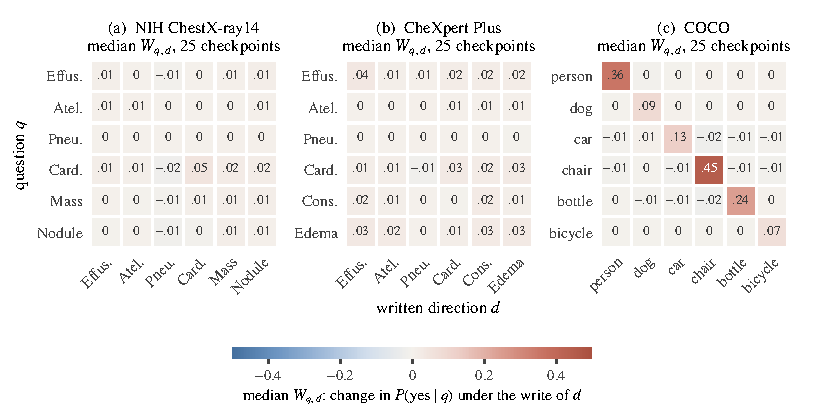
\includegraphics{figures/figA1_write_structure.pdf}}
    \caption{\textbf{Write structure across the grid.} Cell-wise median of the write matrix $W_{q,d}$ over completed checkpoints on NIH ChestX-ray14, CheXpert Plus, and COCO. Figure~\ref{fig:write-flow} reads the same matrices as flow.}
    \label{fig:cf-w-structure}
\end{figure}

\subsection{Per-image examples}
\label{app:cf-examples}

Figure~\ref{fig:cf-examples} shows grades for individual test images, with $P(\mathrm{yes})$ in parentheses on every answer line. The first four chest examples are deficit cells of Qwen2.5-VL-7B, the next two are owned cells (Lingshu 32B Edema, Qwen2.5-VL-72B Atelectasis), and the natural-image examples are owned cells of Qwen2.5-VL-7B, Lingshu 32B, and MedGemma 4B. For a chest example, we pool test rows where the finding is labelled present, the probe reads it (probability above $0.5$), and the clean answer is No. For a natural-image example, we pool rows where the probe reads the label correctly and the clean answer is No. We split each pool by whether the concept's own write or the strongest competing write raises the answer more. Among rows where either write raises the answer by at least $0.2$, we show the row with the gap closest to the median. Each example's last line reports how many pool rows share its ordering, giving the example its own base rate.

\begin{figure}[p]
    \centering
    \resizebox{\textwidth}{!}{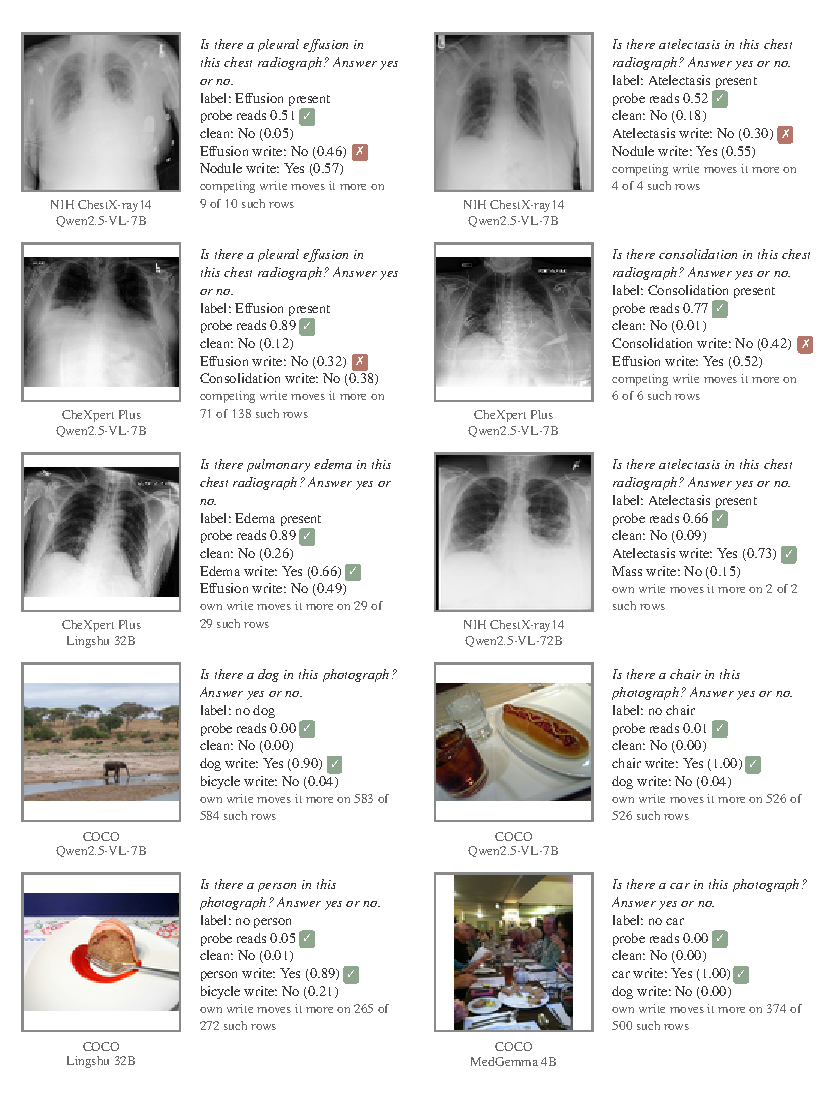
\includegraphics{figures/figA2_examples.pdf}}
    \caption{\textbf{Reading, answering, and writing on single images.} Per image: the question, the report label, the probe's reading, the clean answer, and the answers under the own write and the strongest competing write at $\alpha=+0.25$. Beside the probe's reading, a check or cross marks whether it agrees with the label; beside the own write, whether that write moves the answer more than the competitor. The grey line counts, among the block's test rows the probe reads correctly and the model answers no when clean (on the chest sets, rows labelled present), those with the same ordering.}
    \label{fig:cf-examples}
\end{figure}
